\documentclass[11pt,twoside,a4paper]{book}  
% definice dokumentu
\usepackage[czech, english]{babel}
\usepackage[T1]{fontenc} 				% pouzije EC fonty 
\usepackage[utf8]{inputenc} 			% utf8 kódování vstupu 
\usepackage[square, numbers]{natbib}	% sazba pouzite literatury
\usepackage{indentfirst} 				% 1. odstavec jako v cestine, pro práci v aj možno zakomentovat
\usepackage{fancyhdr}					% tisk hlaviček a patiček stránek
\usepackage{nomencl} 					% umožňuje snadno definovat zkratky a jejich seznam

%%%%%%%%%%%%%%%%%%%%%%%%%%%%%%%%%%%%%%%%%%%%%%%%%%%%%%%%%%%%%%%
% informace o práci
\newcommand\WorkTitle{Návrh a implementace nativní mobilní aplikace pro obchodní zástupce nebankovní společnosti}		% název
\newcommand\FirstandFamilyName{Bc. Jan Hanč}															% autor
\newcommand\Supervisor{Ing. Pavel Malina}															% vedoucí

\newcommand\TypeOfWork{Diplomová práce}	% typ práce [Diplomová práce | Bakalářská práce | Bachelor's Project | Master's Thesis ]	

% Nastavte následují podle vašeho oboru a programu (pomoc hledejte na http://www.fel.cvut.cz/cz/education/bk/prehled.html)								
\newcommand\StudProgram{Otevřená informatika, Magisterský}	% program
\newcommand\StudBranch{Softwarové inženýrství}           					% obor

%%%%%%%%%%%%%%%%%%%%%%%%%%%%%%%%%%%%%%%%%%%%%%%%%%%%%%%%%%%%%%%
% minimální importy
\usepackage{graphicx}					% pro vkládání obrázků
\usepackage{subcaption}
\usepackage{k336_thesis_macros} 		% specialni makra pro formatovani DP a BP
\usepackage[
pdftitle={\WorkTitle},				% nastaví v informacích o pdf název
pdfauthor={\FirstandFamilyName},	% nastaví v informacích o pdf autora
colorlinks=true,					% před tiskem doporučujeme nastavit na false, aby odkazy a url nebyly šedé při ČB tisku
breaklinks=true,
urlcolor=red,
citecolor=blue,
linkcolor=blue,
unicode=true,
]
{hyperref}								% pro zobrazování "prokliknutelných" linků 

% rozšiřující importy
\usepackage{listings} 			%slouží pro tisk zdrojových kódů se syntax higlighting
\usepackage{algorithmicx} 		%slouží pro zápis algoritmů
\usepackage{algpseudocode} 		%slouží pro výpis pseudokódu
\usepackage{wrapfig}
\usepackage{float}
\usepackage{pdfpages}

%%%%%%%%%%%%%%%%%%%%%%%%%%%%%%%%%%%%%%%%%%%%%%%%%%%%%%%%%%%%%%%
% příkazy šablony
\makenomenclature								% při překladu zajistí vytvoření pracovního souboru se seznamem zkratek

\let\oldUrl\url									% url adresy budou zobrazeny: <url> 
\renewcommand\url[1]{<\texttt{\oldUrl{#1}}>}
\renewcommand{\baselinestretch}{1.2}

%%%%%%%%%%%%%%%%%%%%%%%%%%%%%%%%%%%%%%%%%%%%%%%%%%%%%%%%%%%%%%%
% vaše vlastní příkazy
\newcommand*{\nomExpl}[2]{#2 (#1)\nomenclature{#1}{#2}} 	% usnadňuje zápis zkratek : Slova ke Zkrácení (SZ)
\newcommand*{\nom}[2]{#1\nomenclature{#1}{#2}} 			% usnadňuje zápis zkratek : SZ
\lstdefinelanguage{json}{
    basicstyle=\normalfont\ttfamily,
    numberstyle=\scriptsize,
    showstringspaces=false,
    breaklines=true,
	frame=lines,
	inputencoding=utf8,
    extendedchars=true,
    literate=%
    {á}{{\'a}}1
    {č}{{\v{c}}}1
    {ď}{{\v{d}}}1
    {é}{{\'e}}1
    {ě}{{\v{e}}}1
    {í}{{\'i}}1
    {ň}{{\v{n}}}1
    {ó}{{\'o}}1
    {ř}{{\v{r}}}1
    {š}{{\v{s}}}1
    {ť}{{\v{t}}}1
    {ú}{{\'u}}1
    {ů}{{\r{u}}}1
    {ý}{{\'y}}1
    {ž}{{\v{z}}}1
    {Á}{{\'A}}1
    {Č}{{\v{C}}}1
    {Ď}{{\v{D}}}1
    {É}{{\'E}}1
    {Ě}{{\v{E}}}1
    {Í}{{\'I}}1
    {Ň}{{\v{N}}}1
    {Ó}{{\'O}}1
    {Ř}{{\v{R}}}1
    {Š}{{\v{S}}}1
    {Ť}{{\v{T}}}1
    {Ú}{{\'U}}1
    {Ů}{{\r{U}}}1
    {Ý}{{\'Y}}1
    {Ž}{{\v{Z}}}1
}



%%%%%%%%%%%%%%%%%%%%%%%%%%%%%%%%%%%%%%%%%%%%%%%%%%%%%%%%%%%%%%%
% vlastní dokument
%%%%%%%%%%%%%%%%%%%%%%%%%%%%%%%%%%%%%%%%%%%%%%%%%%%%%%%%%%%%%%%
\begin{document}
	
	%%%%%%%%%%%%%%%%%%%%%%%%%% 
	% nastavení jazyka, kterým je práce psána
	\selectlanguage{czech}	% podle jazyka práce nastavte na [czech | english]
	\translate				% nastaví české nebo anglické popisy (např. katedra -> department); viz k336_thesis_macros

	%%%%%%%%%%%%%%%%%%%%%%%%%%    
	% Poznamky ke kompletaci prace
	% Nasledujici pasaz uzavrenou v {} ve sve praci samozrejme 
	% zakomentujte nebo odstrante. 
	% Ve vysledne svazane praci bude nahrazena skutecnym 
	% oficialnim zadanim vasi prace.
	{
	\pagenumbering{roman} \cleardoublepage \thispagestyle{empty}
	\includepdf{zav_prace}

	
	\newpage
	}

	%%%%%%%%%%%%%%%%%%%%%%%%%  
	% Titulni stranka / Title page 
	\coverpagestarts

	%%%%%%%%%%%%%%%%%%%%%%%%%%%    
	% Poděkovani / Acknowledgements 

	\acknowledgements
	\noindent
	Děkuji svému vedoucímu práce panu Ing. Pavlu Malinovi, za konzultace
	a odborné vedení. Dále bych chtěl poděkovat své přítelkyni a rodině za jejich podporu
	při studiích.\\
	\noindent 
	Děkuji také společnosti Provident Financial s.r.o. za poskytnutí nezbytných informací a zdrojů potřebných pro napsání této práce.


	%%%%%%%%%%%%%%%%%%%%%%%%%%%   
	% Prohlášení / Declaration 

	\declaration{V~Praze dne 25.\,5.\,2018}


	%%%%%%%%%%%%%%%%%%%%%%%%%%%%    
	% Abstrakt / Abstract 
 
	\abstractpage

	This thesis deals with design and implementation of a mobile application for the non-banking company. The app is intended for business representatives who visit clients and write contracts, offer additional products and choose installments. A sales representative needs to know the information about the client, so they need to keep them together, so this application helps them. Offers basic statistics, client lists, and forms to fill in. It also provides him with the necessary tools to make it easier to work with the customer.\\
\\\\
	Key words: React native, native application, Application Analysis and Design, Application Development, Marketing
	% Prace v cestine musi krome abstraktu v anglictine obsahovat i
	% abstrakt v cestine.
	\vglue60mm

\newpage
	\noindent{\Huge \textbf{Abstrakt}}
	\vskip 1.75\baselineskip

	\noindent

	Tato práce se zabývá návrhem a implementací mobilní aplikace pro nebankovní společnost. Aplikace je určena obchodním zástupcům, kteří navštěvují klienty a sepisují s nimi smlouvy, nabízejí další produkty a vybírají splátky. Obchodní zástupce potřebuje znát informace o klientovi, takže je potřebuje mít stále při sobě, tedy tato aplikace mu k tomu dopomáhá. Nabízí základní statistiky, seznamy klientů a formuláře k vyplnění. Také mu poskytuje potřebné pomůcky k jednodušší práci se zákazníkem.\\
	\\\\
	Klíčová slova: React native, nativní aplikace, analýza a návrh aplikace, vývoj aplikace, marketing aplikace
	\noindent

	%%%%%%%%%%%%%%%%%%%%%%%%%%    
	% obsahy a seznamy
	\tableofcontents		% Obsah / Table of Contents 

	% pokud v práci nejsou obrázky nebo tabulky - odstraňte jejich seznam
	\listoffigures			% Obsah / Table of Contents 
	%\listoftables			% Seznam tabulek / List of Tables

	%%%%%%%%%%%%%%%%%%%%%%%%%% 
	% začátek textu  
	\mainbodystarts

\chapter{Úvod}
Tato diplomová práce se zaměřuje na obchodní zástupce (nebo také agenty) společnosti Provident Financial s.r.o. (dále společnost), kteří mají za úkol kontaktovat stávající i potencionální zákazníky, sepisovat s nimi smlouvy, poskytovat půjčky a vybírat splátky.

Aplikace, kterou máme za cíl vyvinout, má obchodním zástupcům zjednodušit práci, zefektivnit jí a dosáhnout tak lepších zisků pro společnost. Hlavním cílem aplikace je, aby agent nedělal práci navíc a mohl se dále věnovat svým úkolům. Do aplikace by měl vyplnit údaje jen jednou, a ty se propíší nadále do ostatních systémů, procesů a aktivit, aby mohl stihnout za stejnou dobu, více zákazníků a tím zvýšil nejen své zisky, ale i zisky pro společnost. Zároveň se aplikace bude snažit splnit požadavky obchodu na to, aby agent byl informován o svých výsledcích.

Nejprve zanalyzujeme stávající aplikaci, poté navrhneme řešení pro novou aplikaci a na závěr ji vyvineme. Aplikaci necháme průběžně testovat uživateli, kteří ji budou v budoucnu používat v provozu.

\section{O společnosti}
Společnost Provident Financial s.r.o. působí na českém trhu již od roku 1997 a od té doby její služby využilo více než jeden milion zákazníků. Transparentně nabízí bezúčelové hotovostní i bezhotovostní půjčky, bez ručitele a bez skrytých poplatků. Mezinárodní skupina International Personal Finance (IPF), do níž patří i česká pobočka Provident Financial s.r.o., působí ve Velké Británii již od roku 1880. IPF v současnosti poskytuje služby ve dvanácti zemích světa: v České republice, Polsku, Maďarsku, Rumunsku, Bulharsku, Finsku, Estonsku, Lotyšsku, Litvě, Španělsku, Austrálii a v Mexiku. Jako jedni z prvních poskytovatelů půjček, získali licenci od ČNB, která je zárukou důvěryhodnosti, transparentního financování i odborné způsobilosti a potvrzuje silné postavení na českém finančním trhu. \cite{provident}

\section{Popis práce obchodního zástupce}
Obchodní zástupce je osoba, kterou si určila společnost, jako zástupce pro kontakt se zákazníkem. Tato osoba má v náplni práce aktivně vyhledávat potencionální zákazníky se zájmem o půjčku, informovat zájemce o všech podmínkách, které musí splnit, pro získání půjčky a následně jej provést celým procesem žádosti a sjednání půjčky. 

Po vyplacení (podepsání smlouvy a předání sjednaného obnosu), se nový zákazník stává členem portfolia obchodního zástupce. Zástupce pro své portfolio klientů zajišťuje servis v podobě pravidelných návštěv, kde od zákazníků vybírá splátky na jejich hotovostní zápůjčky a informuje zákazníky o novinkách ve společnosti a možnostech dalšího financování, nebo řeší jakým způsobem srovná zákazník případné nedoplatky, pokud se dostane do prodlení. 

Nedílnou součástí práce obchodního zástupce jsou i retenční nabídky, a to jak před doplacením, tak u zákazníků, kteří již zaplatili veškeré závazky vůči společnosti.

Každý obchodní zástupce má přehled o svých klientech. Seznam těchto klientů má ve svých seznamech, které dostává v tištěné podobě do svých rukou od svého nadřízeného. Nadřízenému se říká manažer a je zodpovědný za více agentů. Skupina, do které patří všichni jeho agenti se nazývá agentura a zároveň je to oblast, kterou má tento manažer na starosti. Manažer si se zástupci dává pravidelná setkání, kde si domlouvají další postupy a manažer pro ně připravuje další materiály pro práci.

\chapter{Analýza}
V této části se pokusíme shrnout aktuální řešení, které ve společnosti existuje, dále se budeme věnovat práci Obchodního zástupce a provedeme mezi nimi průzkum. Průzkumem zjistíme hodnocení aktuální aplikace, poté sestavíme seznam funkčních a nefunkčních požadavků k požadované aplikaci. 

\section{Aktuální řešení}
Tato část se zaměřuje na popis stávající aplikace, použité technologie a funkcionality, které jsou v aktuální aplikaci použity. 

\subsection{Popis}
Současná aplikace \uv{OZ Cockpit} (OZ = Obchodní Zástupce), která slouží obchodním zástupcům ve věci kontaktu se zákazníkem, byla vyvinuta na počátku roku 2016 jedním z kolegů a stala se tak první a jedinou aplikací ve společnosti napříč všemi trhy. Prvotní verze aplikace uměla pouze přihlášení do aplikace pomocí uživatelského jména a hesla. Jméno bylo osobní číslo a heslo telefonní číslo. Aplikace uměla zobrazit pouze vstupní pole pro skóringovou zprávu. Přihlášení probíhalo tak, že uživatel byl po zadání těchto informací ověřen v databázi přes Simple Object Access Protocol\footnote{protokol pro výměnu zpráv ve formátu XML přes síť} (SOAP) službu, a pokud se informace shodovaly, byla odpověď o přihlášení kladná, byl vpuštěn. Omezením bylo to, že při přihlášení se odesílalo i unikátní číslo mobilního telefonu (IMEI), které se uložilo v databázi a žádný jiný telefon se poté nemohl přihlásit pod tímto uživatelem.

První aplikace uměla také, jak již bylo řečeno, odesílat tzv. skóringovou zprávu. Ta slouží k ověření zákazníka v Registru dlužníků a v dalších systémech, které určují, jestli má zákazník nárok na půjčku. Tato zpráva se skládá z parametrů o zákazníkovi, jako je jméno, rodné číslo, měsíční příjmy a výdaje, požadovaná výše půjčky a další nezbytné údaje. Tyto údaje jsou také, v případě kladné odpovědi ze systémů ověřující bezdlužnost (že zákazník má nárok na půjčku), odeslány do interního systému, který vypočítá maximální možnou výši a typ půjčky, kterou mu agent může nabídnout. Tyto informace se opět odesílají zpět na telefon agenta formou textové zprávy. 

\begin{wrapfigure}[15]{r}{0.25\textwidth}
    \centering
	\setlength\intextsep{0pt}
	\includegraphics[width=0.25\textwidth]{figures/oldVersion.png}
	\caption{Vylepšená aplikace}
    \label{fig:betterapp}
\end{wrapfigure}

Po několika vylepšeních aplikace, ke stavu dne 1.1.2018, umožňuje aplikace přihlášení agenta stejným způsobem jako první verze, vyplnění skóringového, výsledkového formuláře a formuláře pro dohodu o snížených splátkách. Výsledkový formulář je soubor polí, které agent denně vyplňuje a odesílá svému nadřízenému. Pole obsahují informace o počtech uzavřených smluv, vybraných částkách atp. Dohoda o snížených splátkách informuje nadřízeného o tom, že zákazník v tuto chvíli nemá na zaplacení splátky a požaduje odložení splátek. Agent se se zákazníkem dohodne a informuje tímto nadřízeného. Ve zprávě se odesílá zákaznické číslo, dohodnutá splátka a den splátky. Tyto informace z formulářů se po stisknutí tlačítka „Odeslat“ odešlou v daném formátu svému nadřízenému či do integračních systémů. 

Další funkcionalitou je zobrazování aktuálních nabízených produktů. Nevýhodou tohoto řešení je to, že aplikace produktovou tabulku obsahuje v kódu. Aplikace ještě ve stavu implementace této funkcionality neměla žádný backend, mimo samotného přihlašování. Stejně tak předpis pro formuláře, pro skóring a výsledky, je v mobilní aplikaci implementován, a při každé změně je nutná přeinstalace aplikace. Poslední přidanou funkcionalitou je zobrazení obchodních výsledků, které jako první začaly komunikovat s backendovou službou na firemním serveru. Obchodní výsledky jsou informace o tom, jak si agent vede v účtovacím období, jestli plní cíle a kolik mu ještě zbývá do splnění cíle uzavřít smluv, vybrat na splátkách a další informace potřebné v rychlém přehledu. 

\subsection{Technologie}
Jedná se o třívrstvou architekturu, která je rozdělena na prezentační vrstvu (Mobilní aplikaci), obchodní vrstvu (Aplikační server) a datovou vrstvu (Databáze). Na obrázku \ref{fig:architecture} je vidět, jak aplikace komunikuje. Komunikace probíhá pomocí SOAP, nebo REST služeb.

\begin{figure}[ht]
\begin{center}
\includegraphics[width=14cm]{figures/aritecture.png}
\caption{Architektura současného řešení}
\label{fig:architecture}
\end{center}
\end{figure}

\subsubsection{Mobilní aplikace}
K vývoji první verze byl použit Ionic framework v.1, který byl schopen pokrýt požadavky na vyplnění polí, komunikaci se službou na serveru a také byl schopen vytvořit a odeslat textovou zprávu. Aplikace, pro které byl použit tento framework, jsou vyvinuty primárně přes Ionic command line utility (neboli „CLI“) a používají Cordovu na sestavní (build) a na nasazení (deploy) jako nativní aplikaci. Po naprogramování bylo možno tuto aplikaci sestavit do podoby pro tři základní podporované mobilní systémy (Android, iOS a Windows). Aplikace se dále rozšiřovala a v současné době pro další rozšíření přestal tento framework stačit. Nebyl schopen pokrýt další požadavky, a proto byl vývoj v tomto frameworku zastaven. Zároveň již byl vyvinut Ionic framework 2.0, který výrazně změnil a zjednodušil původní verzi, která se dále nerozšiřovala. Lze tedy Ionic framework v.1 považovat za zastaralou technologii. \cite{ionicframework}

\subsubsection{Aplikační server}
K vývoji serverové aplikace, která je umístěna v demilitarizované zóně (DMZ), což je server, který má vystaveny endpointy do internetu, je použit jazyk C\# s využitím ASP.NET Web Aplikace (.NET Framework 4.5.1), která je nasazena na serveru Internet Information Services (IIS). Jedná se o dvě serverové aplikace, první je autorizační, která má jeden endpoint, druhá je služba, ke které lze přistoupit po úspěšném ověření, která poskytuje informace pro agenta. Tento server lze dále rozšiřovat o nové endpointy.

\subsubsection{Databáze}
Pro ukládání dat je využit SQL Server 2008 R2. Na serveru je databáze MS SQL, která se serverem komunikuje pomocí Entity Frameworku. Entity framework je objektově-relační zobrazovač, který umožňuje .NET vývojářům jednodušší práci s relačními databázemi, omezuje velikost napsaného kódu a umožňuje práci s databázovými tabulkami, jako s objekty. \cite{entityFramework}

\subsection{Výhody a nevýhody řešení}
Díky této aplikaci si agent ušetřil mnoho času, vzhledem k tomu, že při vyplnění formuláře je potřeba dbát na přesné pořadí a syntaxi. Aplikace mu ji ověřila a díky tomu se vyvaruje několikanásobné úpravě zprávy a odesílání. Nyní tyto pole stačí vyplnit pouze jednou, vše je zkontrolováno a odesláno již validní. Agent má také přehled o svém aktuálním stavu, který je pro něj motivující, pokud se mu daří plán plnit. S tím souvisí i odměny pro agenta za každou uzavřenou smlouvu a při splnění plánu dostává další bonus.

Aktuální řešení pro potřeby agentů je nedostatečné z důvodu omezené funkčnosti aplikace, která pouze nabízí přihlášení a vyplnění několika z potřebných formulářů. Formuláře nejsou dynamicky rozšiřující, a tedy pro každou úpravu detailu nějakého formuláře, je třeba aktualizovat aplikaci. Další nevýhodou aplikace je produktová tabulka, která je také uložena přímo v aplikaci a pro každou změnu produktů, je třeba aplikaci změnit. Pokud se aplikace změní, je nasazena aktualizace do Google Play a Play Store, kde se uživatelům aktualizuje i po několika dnech. To má za následek, že při odesílání zprávy z neaktualizované aplikace, kde chybí několik polí, vrátí odpověď s tím, že je chybně vyplněn formulář, nebo že agent nabízí zákazníkovi produkt, který již není v nabídce.

\section{Potřeby obchodních zástupců}
Byl proveden průzkum mezi jednotlivými agenty o tom, co vykonávají, a jaké vlastnosti či pomůcky, kdyby měli s sebou, by jim ulehčily práci. Otázky, které byly položeny, byly směřovány na aktuální funkčnost aplikace i na její možné rozšíření. Každá otázka byla ohodnocena body, které stanovilo obchodní oddělení. Body byly převedeny na procentuální ohodnocení, ze kterého byl vypočten průměr.

\subsection{Výsledky průzkumu}
Průzkum byl proveden mezi dvaasedmdesáti obchodními zástupci, kteří vyplnili dotazník a výsledky jsou následující.\footnote{Pozn. Výsledky pod 5 \% nejsou zobrazeny ve vyhodnocení.} 

\begin{itemize}
\item Jak často používáte aplikaci OZ Cockpit? - Možnosti “Několikrát denně” odpovědělo 75 \% uživatelů, 13 \% “Jednou denně” a 10 \% “několikrát týdně”. Z toho vyplývá, že agenti jsou seznámeni s aplikací a dle výsledku se dá usuzovat, že je využívána ve velké míře.  
\item Jak jste celkově spojeni s aplikací? - Možnosti “Velmi spokojeni” odpovědělo 13 \%. Nejvíce, 56 \% agentů odpovědělo že jsou “převážně spokojeni” a 18 \% jsou zástupci, kteří nejsou ani spokojeni, ani nespokojeni. Důvody s nespokojeností jsou v největší míře v rychlosti aplikace. Agenti si také stěžují na funkcionality, které jim chybí. Některé z funkcionalit v aplikaci jsou, ale vzhledem k tomu, že o nich agent neví, lze usuzovat, že agenti nejsou informováni o nových funkcionalitách, nebo je aplikace příliš složitá na používání.
\item Jak hodnotíte spolehlivost? - To, že výsledky nejsou nijak příjemné, je patrné již z první odpovědi. Odpověď “Velmi vysoká spolehlivost” odpovědělo 10 \% uživatelů a druhou možnost “Vysoká spolehlivost” odpovědělo 38 \% uživatelů. Nejvyšší skóre dostalo hodnocení “Ani vysoká, ani nízká spolehlivost”, které obdrželo 49 \%. Toto hodnocení je kvůli tomu, že aplikace ne vždy dokáže správně ověřit vstupní data, která jsou vyplněna v aplikaci, tedy se stane, že při odeslání skóringu se vrátí odpověď o chybně vyplněných údajích.
\item Jak hodnotíte jednoduchost používání aplikace? - Odpověď “Velmi jednoduché používání” označilo 22 \% dotazovaných, 41 \% dotazovaných označilo odpověď “Jednoduché používání” a odpověď “Normální používání” označilo 34 \% dotazovaných. Aplikace je podle výsledků jednoduchá na používání, ale vzhledem k tomu, kolik funkcí uživatelé používají, lze usuzovat, že se v aplikaci ne všichni zcela vyznají.
\item Jak často využíváte jednotlivé funkcionality? - V této otázce byly vyjmenovány jednotlivé funkcionality, které aktuálně aplikace nabízí. Možnosti byly “Velmi často”, “Často”, “Ne moc často” a “Vůbec ne”. Průměrně se funkcionality používají na 57 \% což udává to, že ne všechny funkcionality jsou v aplikaci potřebné, nebo je uživatelé neumí používat. Dle odpovědí na jednotlivé otázky se nejméně používá funkcionalita “Dohoda o snížených splátkách”, na kterou odpovědělo “Vůbec ne” nejvíce uživatelů a celkové hodnocení má pouhých 21 \%. Nejlépe dopadly funkcionality “Skóring” a “Výsledkové zprávy”. Ty byly implementovány první. 
\item Uvítali byste některou z následujících funkcionalit? - Byl poslední z dotazů, kde byl dán seznam šesti funkcionalit, které se plánovaly vyvinout a které byly i součástí obchodních požadavků. Nejvíce dotazovaných by uvítalo funkcionalitu seznamu kontaktů na jejich nadřízené, helpdesk a další. Naopak nejméně by využili funkcionalitu “Kalendáře pro plánování návštěv”. Díky tomuto průzkumu a dohodě s oddělením obchodu, se rozhodlo, jaké funkcionality se budou vyvíjet dále. 
\item Obchodní zástupci byli také dotazováni otevřenými otázkami na to, co jim v aplikaci chybí, co by doplnili, či pokud jsou s nějakou funkcionalitou nespokojeni. Měli napsat svůj komentář. Objevovali se zde komentáře k jednotlivým funkčnostem, ale také k rychlejšímu načítání aplikace. Pro další návrh by tyto připomínky měly být brány v potaz a měly by se aplikovat, či by se jim mělo vyhnout v dalším návrhu.
\end{itemize}

\subsection{Vyhodnocení průzkumu}
Většinu funkcionalit agenti používají, ale ne vždy je hodnotí pozitivně. Spolehlivost není na nejlepší úrovni, což může být použitou technologií, či vysokou náročností aplikace na telefon. Vzhledem k tomu, že v aplikaci uživatelům chybí nějaké doplňky, bylo rozhodnuto, že aplikace nedostačuje aktuálním potřebám agentů a je potřeba ji změnit. Je potřeba zjednodušit celou aplikaci, protože ne vždy uživatelé vědí, co se k čemu používá a potřebuje.

\section{Business požadavky}
Požadavky na aplikaci byly stanoveny jednotlivými obchodními manažery, kteří se vyjádřili k tomu, které funkce jsou v aplikaci navíc, a které jim tam chybí. Odpovědi byly rozděleny do dvou kategorií. První kategorie se zabývá technickými funkcionalitami, kterým by měla aplikace odpovídat bez zobrazení jednotlivých oken. Druhá kategorie je požadovaný seznam oken a jednotlivých obchodních požadavků, které informace, nebo pole by měla aplikace poskytovat. 

Aplikace bude určena agentům, kteří se budou setkávat se zákazníky. Musí být bezpečná a reakce na požadavek musí být rychlá. Také musí být přehledná, aby uživatel měl vždy přehled o jednotlivých možnostech aplikace.

\subsection{Nefunkční požadavky}
Seznam nefunkčních požadavků je soupis vlastností aplikace, které bude splňovat bez ohledu na počet zobrazených oken.

\subsubsection{Offline}
Pokud uživatel bude v oblasti, kde není dostatečný přístup k internetu (např. slabý signál), nebo nebude mít v telefonu připojení přes datové připojení, tak se stále musí dostat k informacím o zákazníkovi, které si předem vybere a mít možnost odeslat vyplněné formuláře jinou cestou než přes webové služby, například pomocí textových zpráv. Zobrazení obchodních výsledků, tvaru zpráv, nebo produktů, které jsou aktualizované při dotazu na server, musí být zobrazena poslední známá verze. Tyto informace se aktualizují při dostupnosti datového připojení.

\subsubsection{Synchronizace}
Částečná synchronizace dat se provede za jakéhokoli internetového připojení na žádost uživatele, nebo pokud nějaká data potřebuje načíst aktuálně. Jsou to převážně informace nutné pro prvotní načtení aplikace, nebo informace, které nejsou náročné na spotřebu dat.

Úplná synchronizace dat ze zařízení se provede automaticky při připojení k Wi-Fi síti, kvůli šetření mobilních dat. Aktualizují se informace o zákaznících a produkty. Uživatel by měl mít možnost nastavit si sám, jestli dovolí aplikaci automaticky aktualizovat tyto informace při datovém připojení.

Agenti mají firemní tarif, který obsahuje 1,5GB mobilních dat měsíčně, tedy velikost synchronizace pro jeden dotaz přes mobilní data, nesmí přesáhnout 1MB.

\subsubsection{Logování}
Logování je nutné k případnému zjištění chyb, či běhu aplikace. Logování je prováděno automaticky a v případě výskytu chyby se automaticky odešle zpráva na podporu, která zaeviduje incident a postoupí jej dále k řešení. V logu musí být patrno, jaké kroky uživatel provedl, než se stala chyba, tedy log musí mít historii.

\subsubsection{Zabezpečení}
Požadavek na bezpečnost je nutnost, neboť se pracuje s citlivými daty o zákaznících. Je tedy potřeba zajistit, aby osoba, která není oprávněná tyto data zobrazit, se k nim nedostala. Dále je potřeba mít možnost data na dálku odstranit v případě, že by došlo ke ztrátě nebo odcizení mobilního telefonu agenta.

Přenos na server musí být šifrovaný přes OpenSSL a odesílaný protokolem HTTPs, protože komunikace mezi aplikací a serverem může být odposlouchávána a informace zneužity. 

\subsubsection{Provázanost na jiné aplikace}
Aplikace musí podporovat funkci mapy, která po požadavku na zobrazení adresy bydlištš na mapě, zobrazí pozici uvedené adresy. 

Odesílání textových zpráv z telefonu je nutností z důvodu skóringu nebo reportingu, při kterém je potřeba, aby se zpráva sestavila do přesně stanoveného formátu a byla odeslána na určité telefonní číslo. Tyto informace jsou za normálních okolností odeslány přes webovou službu, ale v případě nedostupnosti služby, je nutné je odeslat jiným způsobem.

Další funkcí, kterou musí aplikace podporovat je přímé vytáčení. Tedy volání po vybrání telefonního čísla, a požadavku na vytáčení. Je potřeba zajistit vyplnění telefonního čísla pro přímé volání. 

\subsection{Funkční požadavky}
Zde si popíšeme chování a jednotlivé požadavky na okna aplikace od obchodního oddělení. Tyto okna se mohou zobrazovat, nebo nemusí, v závislosti na nastavení v databázi pro konkrétní uživatele nebo skupiny. Toto nastavení se odesílá při prvním otevření aplikace, nebo při aktualizaci. Následující usecase \ref{fig:usecase}, popisuje interakci uživatele (agenta) s aplikací a  interakci aplikace se servery.

\begin{figure}[ht]
	\begin{center}
	\includegraphics[width=14cm]{figures/usecase.png}
	\caption{Případy užití aplikace}
	\label{fig:usecase}
	\end{center}
	\end{figure}

\subsubsection{Po spuštění} 
Při prvním otevření aplikace, nebo při odhlášení z aplikace, se uživateli zobrazí okno pro přihlášení. Přihlášení bude prováděno pomocí čísla agenta a telefonního čísla uživatele. Ověřovací zprávou na uvedené telefonní číslo se odešle potvrzovací kód ze serveru, který po zadání do aplikace povolí vstup agentovi k poskytovaným informacím.

V případě špatného zadání, aplikace umožní uživateli změnit vstupní data a zkusit se znovu přihlásit.

Aby se agent přihlásil do aplikace, musí být připojen k internetu, buď na Wi-Fi nebo datovým připojením. Platnost přihlášení bude nastavena na 28 dní a poté dojde k automatickému odhlášení.

\subsubsection{Osobní informace}
Na úvodní obrazovce se zobrazí informace o agentovi (Jméno, příjmení, sekce a pobočka). Agent zde bude mít možnost vidět také Obchodní výsledky, kde bude zobrazen plán a aktuální výsledek pro každou kategorii. Každý agent může mít své kategorie výsledků, které chce jeho nadřízený zobrazovat. Je potřeba zajistit, aby se tyto kategorie zobrazovaly dynamicky. Každá kategorie bude obsahovat název, plán a realitu.

\subsubsection{Skóring}
Aplikace zobrazí obrazovku, ve které budou možnosti vkládání textu, přepínače a jiné podporující funkce, které dopomohou agentovi k jednoduššímu zadávání a automatickému ověřování. Pole pro vyplnění dostane aplikace ze serveru na žádost. Informace ze serveru obsahují popis pole, typ pole (přepínač ANO/NE, checkbox atd.), index pořadí v případě odeslání přes textovou zprávu a ID pole, které označuje klíč v JSON požadavku na server.

Skóring je po stisku tlačítka \uv{Odeslat skóring} odeslán přes internetové připojení na server ke zpracování. Toto se provede pouze pokud je agent připojen k internetu. Pokud agent nemá aktuálně přístup k internetu, je odeslána textová zpráva ve správném formátu.

Formát textových zpráv je posloupnost jednotlivých polí dle svého indexu, oddělena mřížkou. Na začátek je vždy připsán text \uv{\#SCOR\#}, aby bylo poznat, že se jedná o skóringový typ zprávy. \footnote{Příklad skóringové zprávy: \#SKOR\#Jan\#Hanč\#9302221212\#20000\#3000\#45000\#A}

\subsubsection{Produktová tabulka}
Produktová tabulka slouží agentovi jako přehled možných nabízených produktů. Vzhledem k tomu, že se produkty velmi často mění, je potřeba zajistit dynamické vyplnění těchto údajů v aplikaci. Data do aplikace se dostanou z připravené webové služby, která poskytne název tohoto produktu a případně jeho detail. 

\subsubsection{Přehled zákazníků a jejich detail}
V tomto okně se zobrazí seznam zákazníků spadajících pod tohoto agenta. Na první pohled je potřeba rozeznat klienta, kterého si potřebuji zvolit a případně zobrazit jeho detail. K tomu je potřeba v seznamu (pro každého zákazníka) vidět jeho jméno a příjmení, zákaznické číslo a kontaktní adresa. Každý zákazník má své unikátní zákaznické číslo, které se používá pro další zobrazení detailů zákazníka.

Detail zákazníka je obrazovka, kde bude vidět jeho trvalá a kontaktní adresa, telefon, datum narození a celková dlužná částka. Tento detail se musí zobrazit po klepnutí na jednotlivého zákazníka. Je potřeba, aby detaily o zákaznících nevyužívaly velké množství mobilních dat, pokud to nebude nutné, nebo vyžádané uživatelem, neboť agenti mají k dispozici v terénu omezený objem mobilních dat.

\subsubsection{Seznam kontaktů}
Na základě pozice přihlášeného uživatele, tento seznam zobrazuje nadřízeného a ostatní agenty ve skupině. Zároveň zde budou zobrazeny kontakty na Helpdesk a oddělení pro jinou podporu. Společný telefonní seznam je potřeba dynamicky měnit. Každý kontakt bude obsahovat jméno a telefonní číslo.

Tento seznam agent využije například v případě, že nastanou nějaké problémy, nebude si vědět rady, nebo bude potřebovat kontaktovat svého nadřízeného.

\subsubsection{Reportování}
Každý den agent odesílá informace svému nadřízenému o svých výsledcích z aktuálního dne. Opět je nutno, jako ve skóringové zprávě, aby agent mohl jednotlivé parametry vyplnit jednoduše a některé (pokud jsou dostupné), mohly být předvyplněny místo něj a on by pouze zkontroloval, jestli je vše v pořádku a odeslal report.

Parametry, které agent musí vyplnit jsou parametry, které nastaví jeho nadřízený. Ze serveru se posílají informace, které obsahují seznam parametrů nastavených nadřízeným. Položka seznamu obsahuje název parametru, typ vyplňovaného pole (Text, číslo, ANO/NE, a další), index v případě odeslání textové zprávy a ID pole, které označuje klíč v JSON požadavku na server.

Report se odešle požadavkem na server, pokud je agent připojen k internetu. Pokud agent nemá aktuálně přístup k internetu, je odeslána textová zpráva v předem daném formátu. Formát textových zpráv je posloupnost jednotlivých polí dle svého indexu, oddělena mřížkou. Na začátek je vždy připsán text \uv{\#RES\#}, aby bylo poznat, že se jedná o výsledkovou zprávu. \footnote{Příklad výsledkové zprávy: \#RES\#3\#2\#22\#20000\#21400\#45000}

\chapter{Návrh řešení}
V této kapitole se budeme zabývat návrhem řešení aplikace. Design aplikace zpracujeme pomocí programu “Just In Mind (Free)”, který má omezené vlastnosti a funkce oproti plné verzi, kterou jsme si nevybrali, protože je placená a pro studenty není dostupná zdarma. Také si zde zobrazíme jednotlivé obrazovky a popíšeme jejich funkčnosti. Návrh nefunkčních požadavků zpracujeme a popíšeme navrhované řešení.

\section{Návrh nefunkčních požadavků}
Provedeme návrh řešení nefunkčních požadavků, aby splňovaly nefunkční požadavky z analýzy.

\subsection{Ukládání dat do mezipaměti}
Ukládání do mobilního zařízení, je řešeno pomocí interní paměti. Ukládání je v podobě klíč-hodnota do paměti telefonu. Veškeré nastavení nesmí být ukládáno do externí paměti z důvodu snadného přenosu informací do jiných zařízení. Tato paměť bude fungovat jako zdroj informací a nastavení, pokud server nebude k dispozici. Informace poskytující jsou například poslední známé obchodní výsledky, seznam oken a další.

\subsection{Synchronizace}
Pro synchronizaci dat používáme dotazování přes Web API využívající rozhraní REST\footnote{Representational State Transfer} které je založeno na jednoduchých HTTP volání. K synchronizaci použijeme metody HTTP pro webové služby, které spadají do kategorie \uv{RESTful}, tedy GET, POST, PUT a DELETE. Výhody REST komunikace oproti SOAP komunikace spočívají hlavně v objemu dat. K omezení objemu dat také přispěje zapnutí GZIP komprese přenášených zpráv ze strany IIS. \cite{rest}

Synchronizaci rozdělíme do tří typů. Tyto typy od sebe oddělují druh připojení k internetu a závažnost obsahových informací. Tyto typy se snaží brát v potaz množství dat, které může agent měsíčně použít a velikost úložného místa v telefonu, které omezuje část \ref{sec:request}. 

\subsubsection{Bez ohledu na připojení}
Pro správný běh aplikace je potřeba mít přístup k internetu při přihlašování a poté pro prvotní běh aplikace. Po přihlášení je potřeba stáhnout nastavení aplikace, které zaručuje správný běh této aplikace a to, že uživatel opravdu uvidí pouze obrazovky a nastavení, které je mu dovoleno. Tyto informace jsou stahovány bez ohledu na to, jestli je uživatel připojen k síti Wi-Fi, nebo pomocí datového připojení. Tyto informace jsou ukládány do lokální paměti a načteny v případě nedostupnosti internetového připojení. V případě dostupnosti, jsou data aktualizována při zapnutí aplikace.

V tomto režimu nastavení se počítá, že se jedná o požadavky na nastavení, oken aplikace, zobrazování obchodních výsledků a tvar skóringových a výsledkových polí. Počítá se, že tyto informace jsou buď velmi důležité, nebo velmi malé na objem přenesených dat.

\subsubsection{S ohledem na připojení}
Při ohledu na připojení je potřeba vzít v úvahu velikost přenášených dat. Data, která jsou potřeba pro zobrazení základních informací o klientech, nebo kontakty, jsou náročná na objem přenesených dat. Vzhledem k velikosti a počtu, jsou stažena nebo aktualizována okamžitě při připojení k Wi-Fi, protože pro agenta jsou důležitá. Při datovém připojení je na uživateli, zda povolí stahování těchto informací. Data jsou uložena v lokální paměti a načtena při otevření příslušného okna. Pokud je při otevření příslušného okna dostupné připojení k Wi-Fi, je automaticky stažena aktualizace.

\subsubsection{Na požádání} \label{sec:request}
Data, která uživatel nepotřebuje do té doby, dokud se neplánuje setkat s klientem, může si později požádat o stažení do paměti. Data nejsou automaticky stahována ani aktualizována, ale pokud uživatel ví, že za klientem půjde a bude potřebovat jeho detail, může si data o zákazníkovi stáhnout. Pokud uživatel zadá požadavek na stažení detailu klienta při připojení k Wi-Fi, tyto informace se stáhnou bez dotazu. Pokud uživatel bude připojen pouze k datovému připojení bude dotázán, jestli si přeje tyto informace přes toto připojení stáhnout. Možnost nastavení stahování bez dotázání je umožněna v nastavení aplikace. Data v zařízení jsou uložena pouze dočasně po dobu 72 hodin kvůli šetření místa v paměti telefonu a bezpečnosti v případě ztráty zařízení.

\subsection{Logování}
Pro uchovávání logování se bude využívat logování do konzole, které pomocí funkcionalit bude zachytávat doplněk Firebase, který po vyhodnocení chyby, připraví report pro odeslání na administrátory či helpdesk. 

Druhou možností je implementace vlastního loggeru, který bude fungovat na podobné bázi jako Firebase. Tato funkcionalita musí splňovat ukládání chybových hlášení a následné odeslání na server, při dostupnosti internetového připojení.

\subsection{Zabezpečení}
Pro přihlašování do aplikace, se používá dvoufázová autentizace Oauth2 (obr. \ref{fig:oauth2}). Nejprve probíhá ověření, jestli uživatel má právo přistoupit k citlivým datům. Uživatel bude nejprve ověřen odesláním autentizačních informací na server, na základě kterých se jako odpověď vrátí autorizační token. V případě správně vyplněných údajů, se ze serveru na telefonní číslo agenta odešle textová zpráva s vygenerovaným klíčem. Tento klíč uživatel zadá do aplikace a společně s autorizačním tokenem se odešle na autorizační server. Server ověří, jestli token a klíč souhlasí. V případě shody, vrátí uživateli přístupový token (bearer), který umožní uživateli přístup k chráněným informacím. V případě jakékoli neshody, uživatel musí začít znovu.

\begin{figure}[ht]
\begin{center}
\includegraphics[width=14cm]{figures/oauth2.png}
\caption{Oauth2 autentizace}
\label{fig:oauth2}
\end{center}
\end{figure}

Informace uložené v interní paměti musí být šifrované šifrou AES-256 (Advanced Encryption Standard), která poskytuje dostatečné zabezpečení pro ukládání dat. Zároveň se při odhlášení z aplikace, musí lokální paměť smazat, aby se k informacím nedostal žádný jiný uživatel. 

\subsection{Spolupráce s jinými aplikacemi}
V případě kontaktu se zákazníkem musí tato aplikace umět využívat i jiné aplikace, které jsou již vyvinuty a na telefonu standardně nainstalovány. Každý operační systém má své předdefinované aplikace, které umí využít. Těchto aplikací se budeme snažit využít.

\subsubsection{Odesílání textových zpráv}
V případě nedostupnosti internetového připojení, je potřeba skóring a reporty odeslat pomocí textové zprávy. Odesílání skóringu a reportu bude prováděno automaticky pokud to systém bude umožňovat. Operační systémy iOS mají omezení v odesílání zpráv z cizích zdrojů. V tomto případě zpráva bude sestavena a připravena v poli pro odeslání. Odeslat ji musí uživatel manuálně sám.

Agent má v systému registrované pouze jedno telefonní číslo, ze kterého mu je dovoleno odesílat tyto zprávy. Pokud aplikaci používá na jiném mobilním čísle a odešle skóring, nebude platný a automaticky obdrží odpověď, že jeho telefonní číslo není v systému nalezeno.

\subsubsection{Přímé volání}
Seznam kontaktů, nebo informace o zákazníkovi, obsahují informaci o telefonním čísle. Na toto telefonní číslo lze odesílat zprávy a lze na ně také volat. Aplikace musí dovolit přesměrování na výchozí aplikaci pro volání a předat jí toto telefonní číslo, které uživatel chce vytočit.

\subsubsection{Mapy}
Pokud se agent rozhodne kontaktovat zákazníka osobně, uvítá možnost \uv{Zobrazení na mapě}, která zobrazí adresu zákazníka ve výchozí aplikaci na mapě. Pokud taková aplikace v telefonu neexistuje, zobrazí se adresa na mapě Google na webové stránce v okně prohlížeče.

\section{Návrh funkčních požadavků}
Zde popíšeme a ukážeme jednotlivé zpracování funkčních požadavků aplikace. Ke každé funkcionalitě je přiřazena obrazovka, která popisuje požadovanou funkci. Návrh obrazovek je tvořený pro mobilní telefon Nexus 5S.

\subsection{Přihlášení}
Obrazovka \ref{fig:loginscreensa} se objeví jako první po spuštění aplikace. Tato obrazovka bude obsahovat dvě textová pole pro zadání přihlašovacích údajů. První na osobní číslo, druhé na telefonní číslo. Po vyplnění požadovaných údajů na úvodní stránce, dojde k odeslání požadavku na server a v případě kladné odpovědi, je obrazovka vyměněna za druhou obrazovku \ref{fig:loginscreensb}, kam uživatel zadá ověřovací kód, který mu byl zaslán na jeho telefonní číslo. Při vyplnění správného čísla, přejde aplikace na úvodní stránku \ref{fig:initscreensa}.

\begin{figure}[hbp]
	\centering
	\begin{subfigure}{.3\textwidth}
	  \centering
	  \includegraphics[width=.66\textwidth]{figures/Design/login.PNG}
	  \caption{Základní přihlášení}
	  \label{fig:loginscreensa}
	\end{subfigure}%
	\begin{subfigure}{.3\textwidth}
	  \centering
	  \includegraphics[width=.66\textwidth]{figures/Design/loginsecurity.PNG}
	  \caption{Ověřovací číslo}
	  \label{fig:loginscreensb}
	\end{subfigure}
	\begin{subfigure}{.3\textwidth}
		\centering
		\includegraphics[width=.66\textwidth]{figures/Design/loginfailde.PNG}
		\caption{Chybné údaje}
		\label{fig:loginscreensc}
	\end{subfigure}
\caption{Okna přihlašování do aplikace}
\label{fig:loginscreens}
\end{figure}

Pokud na první obrazovce přihlašování nastane chyba, uživateli se objeví obrazovka s chybou \ref{fig:loginscreensc}, která oznamuje uživateli, že zadal nesprávné údaje a celé přihlašování musí začít znovu. Pokud nastane chyba v opisování zprávy, uživatel má možnost 2 oprav před tím, než aplikace zobrazí chybové hlášení a uživatel je přesměrován na první stránku přihlášení.

\subsection{Úvodní obrazovka}
Na úvodní obrazovce, v horní části, je zobrazen název aplikace. Pro rozbalení jednotlivých možností v levém horním rohu se zobrazí překrývající menu, kde je možno zvolit z jednotlivých obrazovek popsaných v kapitole \ref{sec:menuDesign}. 

Obsah první stránky (obr. \ref{fig:initscreensa}) tvoří jméno, příjmení, sekce kterou agent zastupuje a agenturu, ve které působí. Při prvním pohledu do aplikace, uživatel dostane přehled o svých obchodních výsledcích. Tabulka obsahuje výsledky jednotlivých kategorií. V prvním sloupci je název hodnotící kategorie, ve druhém sloupci je plán, který agentovi naplánoval nadřízený a ve třetím sloupci jsou reálné výsledky, kterých dosáhl za poslední zúčtovací období. 

\begin{figure}[ht]
	\centering
	\begin{subfigure}{.4\textwidth}
	  	\centering
	  	\includegraphics[width=.5\textwidth]{figures/Design/init.PNG}
	  	\caption{Úvodní obrazovka}
	  	\label{fig:initscreensa}
	\end{subfigure}
	\begin{subfigure}{.4\textwidth}
	  	\centering
		\includegraphics[width=.5\textwidth]{figures/Design/InitSMS.PNG}
	  	\caption{Výběr nové zprávy}
	  	\label{fig:initscreensb}
	\end{subfigure}
\caption{Úvodní obrazovka po přihlášení do aplikace}
\label{fig:initscreens}
\end{figure}

V pravém spodním rohu je kruhové zelené tlačítko se znakem plus. Pokud uživatel klepne na toto tlačítko, rozbalí se menu nad tímto tlačítkem pro vytvoření nové zprávy jako je možné vidět na obrázku \ref{fig:initscreensb}. Ikona plusu se změní na ikonu křížku, která po klepnutí opět schová toto menu. K dispozici jsou dva druhy zpráv. První druh zprávy je zpráva skóringová se značkou osoby s plusem. Po klepnutí na tuto ikonu, uživatel bude přesměrován na obrazovku skóringu popsanou v kapitole \ref{sec:scoringDesign}. Druhou ikonou je ikona dolaru, která představuje ikonu výsledkové zprávy, popsanou v kapitole \ref{sec:reportDesign}, na kterou se po klepnutí toto okno přesměruje.

\begin{wrapfigure}[11]{R}{0.2\textwidth}
    \centering
	\setlength\intextsep{0pt}
	\includegraphics[width=0.2\textwidth]{figures/Design/initMenu.PNG}
	\caption{Rozbalovací menu}
    \label{fig:menuscreens}
\end{wrapfigure}

\subsection{Rozbalovací menu} \label{sec:menuDesign}
Rozbalovací menu je typem responsivní navigace a je určeno pro rychlou navigaci mezi požadovanými okny. Rozbalovací proto, protože se rozvine (rozbalí) z levé strany obrazovky a překryje obsah. 

Hlavní obrazovky (obrazovky vyjmenované v seznamu) mají v levém horním rohu aplikace zobrazen symbol menu neboli tři vodorovné čárky nad sebou, též označován jako “hamburger menu”. Po kliknutí na ikonu menu, se z levé strany zobrazí menu, které zobrazuje přehled hlavních obrazovek. Toto menu lze také vyvolat přejetím z levé strany obrazovky doprava. Po klepnutí na název požadované funkce se zobrazí její obrazovka. 

V horní části menu, je vidět jméno přihlášeného uživatele následované přidělenými obrazovkami, a dále nastavení aplikace a odhlášení. Tlačítko odhlášení, uživatele odhlásí z aplikace, tedy odstraní token z paměti a vymaže veškerá uložená data o aplikaci.

\subsection{Skóringová zpráva} \label{sec:scoringDesign}
Po klepnutí na stránku skóringu je uživatel požádán o vyplnění veškerých údajů, které jsou potřeba pro správné oskórování zákazníka. To, že vyplněná pole jsou podle požadavků se ověřuje pomocí regulárního výrazu, který každé z těchto polí obsahuje. Pole jsou dynamická, takže jsou stahována přes webovou službu z databáze. Jedná se o pole, která budou textová, numerická, ANO/NE tlačítka s vlastním nastavením textu a výběrové menu z více možností. Pole jsou rozdělena do kategorií pro lepší přehlednost. Všechna jsou povinná. 

Po vyplnění veškerých polí (pokud je vše správně vyplněno), po stisknutí tlačítka “Skórovat”, nebo tlačítka složené papírové vlaštovky v pravém horním rohu, se odešle zpráva sestavená dle požadavků a uživateli se zobrazí potvrzení o úspěšném odeslání zprávy. Pokud je uživatel připojen k internetu jakýmkoli způsobem, odešle se zpráva přes webovou službu, pokud ne, sestaví se do textové zprávy a odešle se. 

V horním panelu uprostřed, je text s názvem okna, v levé části panelu je odkaz na menu \ref{sec:menuDesign}.

\begin{figure}[ht]
	\centering
	\begin{subfigure}{.4\textwidth}
	  	\centering
	  	\includegraphics[width=.5\textwidth]{figures/Design/scoring.PNG}
	  	\caption{Vyplnění údajů}
	  	\label{fig:scoringscreensa}
	\end{subfigure}
	\begin{subfigure}{.4\textwidth}
	  	\centering
		\includegraphics[width=.5\textwidth]{figures/Design/scoringmessage.PNG}
	  	\caption{Informace o odeslání}
	  	\label{fig:scoringscreensb}
	\end{subfigure}
\caption{Obrazovky pro odesílání skóringu}
\label{fig:scoringscreens}
\end{figure}

\subsection{Reportování} \label{sec:reportDesign}
Reporting slouží k odesílání informací o denních výsledcích. Informace, která pole je povinen uživatel vyplnit jsou uložena v databázi a zobrazována jako řádky pod sebou. Každý řádek je jeden parametr pro vyplnění. Parametry pro vyplnění mohou být numerické, textové, nebo pole volby ze dvou, či více možností.

\begin{figure}[ht]
	\centering
	\begin{subfigure}{.4\textwidth}
	  	\centering
	  	\includegraphics[width=.5\textwidth]{figures/Design/report.PNG}
	  	\caption{Pole pro vyplnění}
	  	\label{fig:reportscreena}
	\end{subfigure}
	\begin{subfigure}{.4\textwidth}
	  	\centering
		\includegraphics[width=.5\textwidth]{figures/Design/reportmessage.PNG}
	  	\caption{Oznámení o odeslání}
	  	\label{fig:reportscreenb}
	\end{subfigure}
\caption{Obrazovky pro vyplnění a odeslání výsledků}
\label{fig:reportscreen}
\end{figure}

Na konci řádků pro vyplnění, bude tlačítko pro odeslání výsledků. Toto tlačítko má stejnou funkci jako tlačítko odeslat v pravém horním rohu (znak složené papírové vlaštovky). Po stisku tohoto tlačítka, aplikace zajistí, že se odešle výsledková zpráva, v případě připojení k internetu přes webovou službu, v případě offline provozu se odešle textová zpráva v daném formátu. V případě správného odeslání zprávy, se zobrazí informace o odeslání výsledků. V případě neúspěchu se zobrazí informace, o tom, kde nastala chyba.

V horním panelu uprostřed, je text s názvem okna, v levé části panelu je odkaz na menu \ref{sec:menuDesign}.

\subsection{Produktová tabulka}
Produktová tabulka obsahuje seznam půjček, které společnost aktuálně nabízí a agent je může nabídnout zákazníkovi. Tyto data se stahují přes webovou službu. Agent vidí jména půjček, jejich znak a barvu. Stránka nemá žádné přímé návaznosti na jiné stránky, je pouze zobrazovací.

V horním panelu uprostřed, je text s názvem okna, v levé části panelu je odkaz na menu \ref{sec:menuDesign}.

\begin{figure}[H]
	\centering
	\includegraphics[width=0.2\textwidth]{figures/Design/prod.PNG}
	\caption{Produktová tabulka}
	\label{fig:productscreens}
	\end{figure}

\begin{wrapfigure}[15]{r}{0.2\textwidth}
	\centering
	\includegraphics[width=.2\textwidth]{figures/Design/customer.PNG}
	\caption{Přehled zákazníků}
	\label{fig:customerscreens}
	\end{wrapfigure}
	
\subsection{Přehled zákazníků} \label{sec:customerDesign}
Jako další obrazovkou je zobrazení základních klientských informací. Klienti jsou zobrazeni v jednotlivých řádcích pod sebou. V řádku je zobrazeno jméno klienta a jeho osobní číslo v závorce. Pod jménem klienta je uvedena jeho adresa pro lepší orientaci. Vedle jména zákazníka je checkbox, který označuje, že detail zákazníka je v mobilním zařízení stažen pro použití offline. Zároveň je tento zákazník zachycen na vršek stránky. Datum nad checkboxem označuje datum posledního kontaktu zákazníka.

V horní části obrazovky jsou zobrazeny dvě tlačítka. Jedno aktualizační (zobrazeno jako stočená šipka sama do sebe), které aktualizuje základní informace o zákaznících. Aktualizace je na požádání při datovém připojení i při Wi-Fi připojení. Dále zde je zobrazeno tlačítko filtru (zobrazeno jako tři zmenšující se čárky pod sebou), které po stisku zobrazí vyhledávání zákazníka podle jména, osobního čísla a adresy. Toto vyhledávání není potřeba napsat přesně a celé, stačí napsat jen část a automaticky se vyhledají zákazníci, kteří tento text obsahují.

V horním panelu uprostřed, je text s názvem okna, v levé části panelu je odkaz na menu \ref{sec:menuDesign}.

Každý zákazník obsahuje detail, kde se zobrazují další informace, potřebné pro agenta. K těmto informacím se uživatel dostane tak, že klepne na nějakého zákazníka a automaticky bude přesměrován na jeho detail popsaný v kapitole \ref{sec:custDetailDesign}
\newpage
\begin{wrapfigure}[14]{l}{0.2\textwidth}
	\centering
	\includegraphics[width=.2\textwidth]{figures/Design/custDetail.PNG}
	\caption{Detail zákazníka}
	\label{fig:customerdetailscreens}
	\end{wrapfigure}

\subsection{Detail zákazníka} \label{sec:custDetailDesign}
Do detailu zákazníka se dostane uživatel tak, že na kartě Zákazníci \ref{sec:customerDesign}, klepne na jméno v řádku zákazníka, kterého detail chce zobrazit. Nová stránka s detaily zákazníka, se překryje přes tuto kartu. Zobrazené detaily na této stránce jsou: telefonní číslo, adresa domů a adresa kontaktní, což je adresa, kde se klient vyskytuje, kde ho má agent navštívit. Po stisku tlačítka vedle telefonního čísla vpravo, začne na toto číslo uživatel psát textovou zprávu. Po stisku tlačítka vpravo vedle adresy, se zobrazí tato adresa na mapě. Po klepnutí na telefonní číslo, aplikace toto telefonní číslo vytočí. 

Tlačítkem v pravém horním rohu se aktualizují detailní informace o zákazníkovi, neboli se požádá o nové informace. Tyto informace mohou být zastaralé, pokud jsou v zařízení uloženy delší dobu. Tlačítko v levém horním rohu (šipka směrem doleva), se vrátí zpět na kartu Zákazníci, do hlavního postavení, na vrchol stránky. 
 
\subsection{Kontakty}

Na záložce Kontakty jsou vidět kontakty dvou druhů. Kontakty agentury (na obr. \ref{fig:contactscreensa}) a všechny kontakty (na obr. \ref{fig:contactscreensb}), které jsou agentovi k dispozici. V první záložce "Agentura", jsou kontakty z jeho agentury, do které spadá. Jako první se zobrazí jméno nadřízeného s jeho pozicí, druhý je zde uveden senior agent a další v pořadí jsou zobrazeny ostatní agenti, spadající do stejné agentury, jako přihlášený agent. V druhé záložce "Všechny kontakty" kde jsou navíc kontakty, které mu dopomohou v případě nějakých potíží, jako třeba přímé volání na helpdesk a další. Zároveň jsou zde zobrazeny kontakty z agentury,  zobrazené pod těmito kontakty. 

Ikona telefonu vedle každého kontaktu vytvoří okamžité volání na přidělené telefonní číslo. Ikona zprávy přesměruje uživatele do tvorby textové zprávy, kde předvyplní telefonní číslo kontaktu.

\begin{figure}[H]
	\centering
	\begin{subfigure}{.4\textwidth}
	  	\centering
	  	\includegraphics[width=.5\textwidth]{figures/Design/contacts.PNG}
	  	\caption{Kontakty agentury}
	  	\label{fig:contactscreensa}
	\end{subfigure}
	\begin{subfigure}{.4\textwidth}
	  	\centering
		\includegraphics[width=.5\textwidth]{figures/Design/contactsAll.PNG}
	  	\caption{Všechny kontakty}
	  	\label{fig:contactscreensb}
	\end{subfigure}
\caption{Obrazovka kontaktních informací společnosti}
\label{fig:contactscreens}
\end{figure}

\subsection{Nastavení}
Na obrazovce nastavení si může uživatel zvolit nastavení aplikace. Jednotlivá nastavení zde mohou být vyjmenována, popsána a případně doplňována. Pro tuto verzi, budeme požadovat nastavení stahování informace a to konkrétně, jestli se budou stahovat automaticky informace o zákaznících, v případě připojení přes data. Pokud je zaškrtnuto první políčko \uv{Základní informace o zákaznících}, automaticky se budou načítat informace o zákaznících bez upozornění, že uživatel je připojen k datovému připojení. To stejné se bude dít v případě detailních informací a zaškrtnutí druhého políčka \uv{Detailní informace o zákaznících}. Uživatel tedy dále nebude upozorňován, jestli aplikace může tyto data synchronizovat.

\begin{figure}[H] 
	\centering
	
\includegraphics[width=.2\textwidth]{figures/Design/settings.PNG}
	\caption{Obrazovka nastavení}
	\label{fig:customerdetailscreens}
	\end{figure}


\section{Testování s uživateli}
Návrh aplikace byl vytvořen v programu \uv{Justinmind Prototyper (FREE)}, který umožňuje návrh designu aplikace a přechody mezi jednotlivými obrazovkami. Toto vše mohlo dát dohromady alespoň hrubý návrh aplikace, která přechází mezi jednotlivými obrazovkami a mohli jsme dát vybraným budoucím uživatelům otestovat intuitivnost aplikace na jednotlivých, předem připravených, testovacích scénářích. 

Na testování se podílelo pět budoucích uživatelů. Při testování se měřila rychlost nalezení správné cesty, jestli nalezli všechny cesty a jestli si všimli všech informací a tlačítek na stránce. Jako počáteční stránka byla vždy dána stránka po přihlášení, tedy "Úvodní obrazovka".

\subsection{Vyplňte skóringové informace a odešlete zprávu}
K našemu překvapení, většina uživatelů (4 z 5ti) neprocházela přes menu, které skrývá většinu z oken, ale přes tlačítko, které se nachází v pravém dolním roku a přes něj prvním tlačítkem na skóring. Uživatelé dokázali najít tlačítko k vytvoření zprávy okamžitě, bez rozmýšlení. 

Všichni uživatelé vyplnili zprávu správně. Všichni uživatelé, mimo jednoho, odeslali zprávu na konci stránky, pouze jeden uživatel si všiml a odeslal ji přes tlačítko v pravém horním rohu. Uživatelé, kteří odeslali zprávu přes tlačítko na konci stránky si nevšimli tlačítka v pravém horním rohu, nebo je nenapadlo, že se jedná o stejné tlačítko.

Lidé, kteří otevřeli zprávu přes tlačítko v pravém dolním rohu, pak také dokázali otevřít toto okno přes menu, ale uživatel, který otevřel prvně menu, nebyl schopen najít druhou cestu.

\subsection{Otevření navigace k zákazníkovi}
Uživatelé byli požádáni, aby zobrazili na mapě místo bydliště klienta, který bydlí v Aši. Uživatelé se přes tlačítko menu bez problémů dostali na stránku zákaznického přehledu. Všichni se na první pohled zorientovali na stránce. Pouze tři z nich, po klepnutí na zákazníka, se dostali na detail tohoto zákazníka. Zde se v první chvíli snažili klepnout na text s adresou, po chvíli si všimli znaku navigace a přes toto tlačítko, si její adresu zobrazili. Ostatní se snažili adresu přepsat do aplikace map. Všichni nakonec dokázali poklepat na tlačítko navigace, která by je (v případě funkčnosti) navedla na mapu.

Funkce zobrazení na mapě, by se měla přesunout na celé tlačítko, nejen pod ikonu navigace.

\subsection{Zavolání na helpdesk}
Uživatelé byli požádáni, aby s použitím aplikace našli kontakt na helpdesk a zavolali tam. Všichni neměli problém nalézt kartu s kontakty, ale problém nastal při hledání na kartě, kde kontakt na helpdesk naleznou. Pouze jeden uživatel bez problémů klepl na kartu se všemi kontakty a poté na tlačítko sluchátka u řádku “Helpdesk”. Po zaváhání ostatních se podařilo i jim otevřít druhou záložku a také zavolat přes tlačítko sluchátka. 

Tlačítko sluchátka je natolik intuitivní, že uživatelé neklikali na uživatele, ale přímo na tuto ikonu.

\subsection{Nastavení automatického stahování základních informací o zákaznících přes datové připojení}
V tomto případě byl jednoduchý úkol, který ve výsledku měl za cíl pouze nalézt stránku nastavení a zaškrtnout jedno políčko. Toto se ukázalo jako velký problém, neboť většina uživatelů neporozuměla otázce, ani tomu, proč by něco takového měli chtít nastavovat. Po detailním vysvětlení byli schopni všichni nalézt požadovanou stránku a zaškrtnout správné pole. S tímto úkolem měli uživatelé velký problém. Ukázal se jako nejméně intuitivní.

\subsection{Odhlášení}
Naopak nejvíce intuitivní pro uživatele bylo, odhlášení z aplikace. Všichni okamžitě otevřeli menu a stiskli tlačítko \uv{Odhlásit se}.

\subsection{Shrnutí}
Při testování jsme zjistili, že aplikace potřebuje drobné úpravy, které nejsou vážné. Uživatelé při celkovém hodnocení hodnotili aplikaci jako přehlednou, chválili postranní menu, které uživatelům dopomáhá k lepší orientaci a ocenili tlačítko pro rychlé vytvoření zpráv. 

Když si všimli kategorie nastavení, v první chvíli očekávali, že si zde mohou nastavit jazyk, barvy, zvuky, typy písma a další obecná nastavení. Nastavení, které ale aplikace umožňuje, jim nepřipadalo důležité i po vysvětlení.

Po vysvětlení další funkcionality, a to dynamického zobrazování polí ve skóringové zprávě, reportingu a v produktech, byli uživatelé nadšeni, protože se aplikace nadále nemusí aktualizovat při každé změně. Aktualizace aplikace vždy provázely nějaké problémy, tento přístup jim tedy přišel o hodně snesitelnější.

Uživatelé ocenili obrazovku kontakty, kterou do této chvíle neměli. 

Připomínku měli k obrazovkám zákazníků, kde si stěžovali na částečnou nepřehlednost a nedostatek informací o zákazníkovi. Tyto informace nadále rozšíříme a upravíme řádkování pro větší přehlednost. Doplníme také popisky některých ikon, se kterými měli uživatelé problém. Některé ikony vyměníme za text.

\chapter{Implementace}
V této kapitole si popíšeme technologie, které můžeme použít a zvolíme si jednu z nich. Aplikaci vyvineme a poté popíšeme jednotlivé implementační kroky, které při vývoji aplikace nastaly. Popíšeme také jednotlivé obrazovky, jaké funcionality se podařilo implementovat a jaké ne.

\section{Technologie pro vývoj}
Vzhledem k požadavkům na aplikaci, jakožto vývoj multiplatformní aplikace, jsme si mohli zvolit z nepřeberného množství hybridních technologií. Po výběru nejpoužívanějších s nejlepším hodnocením jsme vybrali tři technologie, které by byly vhodné pro implementaci.\cite{hybridniaplikace}

\subsection{Nativní aplikace}
Nativní aplikace je aplikace, která je vytvořena pouze pro jednu platformu (např. pouze pro iOS nebo pro Android). V případě, že ji chceme mít na jiné platformě, je nutné vytvořit jinou aplikaci, i když může mít shodnou funkcionalitu. 

Výhodou je, že spolupracuje s hardware mobilních zařízení, může pracovat offline a umí lépe využít všech vlastností operačního systému - jsou tedy přirozeně rychlejší a mohou využívat dalších služeb nebo vlastností systému, jako jsou například pohybová gesta, a další.

\subsection{Webová aplikace}
Webové aplikace fungují obvykle na všech platformách jako přizpůsobené www stránky, tedy k provozu je potřeba pouze webový prohlížeč. Data se uchovávají na serveru, a tedy jsou přístupná odkudkoliv. Omezením bývá nižší možnost spolupráce s hardware mobilních zařízení a často je nelze používat offline. Jsou zde i možná bezpečnostní rizika úniku dat v případě nekvalitního poskytovatele.

\subsection{Hybridní aplikace}
Hybridní aplikace je kombinací webových a nativních technologií. Specializované nástroje umožňují vývoj pomocí k tomu určených webových technologií a následné konverze na nativní aplikace pro jednotlivé platformy. 

Tyto aplikace jsou stále populárnější pro svou pohodlnost a rychlost vývoje a pro svou rychlost aplikace jako takové. Dají se vhodně použít pro práci s hardware telefonu, seznamy, propojení se sociálními sítěmi a další. Musí se počítat s pomalejšími časy pro složitější dotazy. Práce s audiem a videem také nepatří k silným stránkám technologie. 

Vzhledem k potřebám, které vyžaduje tato aplikace, jsme si zvolili hybridní technologii k návrhu aplikace. Uvedeme si příklady frameworků a porovnáme, který je pro náš vývoj nejlepší.

\subsubsection{Xamarin}
Xamarin je platforma pro vývoj nativních mobilních aplikací pro platformy iOS, Android, Windows. Aplikace jsou programovány v jazyku C\#/.NET, nebo jazyku F\#. 
Xamarin umožňuje psaní kódu v jednom jazyce, ale také lze využít Xamarin.Forms, které umožní navrhnout UI pro více platform najednou. 

Pro kompilaci využívá Just-in-time (JIT) nebo Ahead-of-time (AOT) kompilaci. JIT nelze použít pro iOS, tedy se využívá AOT. Na ostatních platformách může používat JIT nebo AOT dle nastavení. \cite{cruxlab}

Tato platforma je rozšíření do Visual Studia, které v omezené funkcionalitě je OpenSource. Vývoj je rychlý a kompilace také, avšak vzhledem k C\# kódu je často problém převést do platformy pro Android nebo iOS. 

\subsubsection{Ionic}
Ionic je framework pro vývoj hybridních mobilních aplikací. Kód je psaný v Javascriptu/Typescryptu a také využívá Angular framework a HTML5. Pro zobrazování využívá web view, tedy si s sebou ponese vždy prohlížeč, ve kterém bude zobrazovat uživatelské rozhraní (UI) v HTML. Pro kompilaci využívá JIT. \cite{cruxlab}

Bohužel aplikace napsané v Ionic frameworku se dlouho kompilují a v případě náročnějších (komplexnějších) aplikací a velkým nárokům na start aplikace, je běh samotný také pomalý.

\subsubsection{React Native}
React Native je framework pro vývoj nativních mobilních aplikací, který vyvinul Facebook. Hlavní výhodou technologie React Native je možnost vývoje pouze jednoho sdíleného kódu pro všechny platformy (iOS, Android, web). Kód je psaný v Javascriptu/Typescryptu a pro UI využívá speciální templovací jazyk, kterého je výsledkem vytvoření nativních widgetů. React dokáže detekovat změny a poté překreslit pouze je. Toto může čas kompilace urychlit. \cite{eisenman_2016}

Nespornou výhodou pro vývoj v React Native, je použití velkého množství knihoven, které jsou zdarma a open source. Přidáním knihovny si můžeme nadále rozšířit možnosti s aplikací. Jako typickým příkladem knihovny, která nabízí spoustu komponent, které jsme dále použili v aplikaci, je knihovna Native Base. Tato knihovna nabízí spoustu komponent, které se v aplikaci dají použít a jsou pohodlné na použití, funkční a designově hezké. Příkladem takového kódu je \ref{lst:example}.

\begin{minipage}{\linewidth}
\begin{lstlisting}[caption=Základní syntaxe NativeBase komponenty, label={lst:example}]
import React, { Component } from 'react';
import { Container, Button, Text } from 'native-base';

export default class GeneralExample extends Component {
  render() {
    return (
      <Container>
        <Button>
          <Text>
            ButtonText
          </Text>
        </Button>
      </Container>
    );
  }
}
\end{lstlisting}
\end{minipage}

První dva řádky určují, jaké knihovny se použijí (react a native-base) a jaké se použijí komponenty z knihovny (Container z native-base). Tím se definují a předpokládá se jejich použití v kódu. Třída musí obsahovat "render" metodu. Tato metoda určuje, co se bude zobrazí. Co se bude zobrazovat určí v této metodě return, který v závorkách obsahuje výsledek. V returnu jdou vidět použité komponenty, tedy Container, který obsahuje tlačítko (Button), ve kterém je text (Text), ve kterém se text "ButtonText" zobrazí na tlačítku.

Určitě stojí za zmínku i dynamické vykreslování, které nám dále pomůže dynamicky zobrazovat to, co nám přijde v požadavku na vykreslení. Toto vykreslení by mělo být dynamicky rozšířitelné, tedy je potřeba nějaká funkce, která bude bez ohledu na velikosti, zobrazovat jeho obsah. React Native má tu výhodu, že je to javascriptová aplikace, která umí využívat tuto syntaxi k dalšímu vykreslování. Pokud máme dohodnutý formát v JSON, který nám přijde v odpovědi na požadavek, a máme strukturu do které se obsah bude vykreslovat, lze použít pro dynamické vykreslování funkci \textit{map}. Tato funkce dokáže při zavolání nad objektem vrátit přesně definovanou strukturu pro každý záznam. 

Příklad kódu \ref{lst:dynmap} je dynamické vykreslování řádků do mřížky. V prvním řádku jde vidět prvotní načtení .json souboru, ve kterém je uložen tento záznam, obsahující tři textové řetězce. JSON struktura se převede do objektu, a pak se s ním dále pracuje jako s dynamickým objektem a lze na něj odkazovat. Na takto načtený soubor se zavolá funkce \textit{map}, a jako dva parametry jsou objekt, který to iterovalo (item) a index té iterace (i). Tyto proměnné se poté použijí ve funkci, která vytvoří nové objekty do tagů a do nich vloží tuto hodnotu. Aby bylo patrné, že se jedná o proměnné, musí se vložit do složených závorek. Tato syntaxe vykreslí jednotlivé řádky mřížky.

\begin{minipage}{\linewidth}
\begin{lstlisting}[caption=Dynamické vykreslování obsahu funkcí map,label={lst:dynmap}] 
const example = require("example.json");
	...
render() {
 return (
  <Content>
   <Grid>
   {
    example.map((item, i) => {
      return (
       <Row key={i} >
        <Col><Text style={styles.firstColumn}>{item.text1}</Text></Col>
        <Col style={styles.column}><Text>{item.text2}</Text></Col>
        <Col style={styles.column}><Text>{item.text3}</Text></Col>
       </Row>
      )})
    }
   </Grid>
  </Content>
 );
}
\end{lstlisting}
\end{minipage}

Rozhodně stojí za to si povšimnout stylů. Tyto styly jsou definované mimo tento kód, jako je tomu například u kaskádových stylů. React používá objektového přístupu, tedy ke stylu lze přistoupit jako k objektu. Tyto styly jsou definované v typescriptovém souboru, který je poté využíván. Příkladem takových sylů je \ref{lst:styles}, který definuje styl sloupce.

\begin{minipage}{\linewidth}
\begin{lstlisting}[caption=Příklad nastavení stylů, label={lst:styles}]
export default StyleSheet.create({
 column: {
  height: 24,
  alignItems: 'center'
 },
 firstColumn: {
  fontWeight: 'bold',
 }
});
\end{lstlisting}
\end{minipage}

Ikdyž framework je poměrně nový, má před sebou slibnou budoucnost. Časem své kompilace vysoce převažuje ostatní frameworky a rychlost jeho vývoje je poměrně vysoká, protože jsou potřeba pouze základní znalosti o tom, jak celý framework funguje, a tedy jsme si jej zvolili jako framework pro naší aplikaci.

\section{Prostředí pro vývoj}
K vývoji aplikace v React Native, je potřeba si zvolit vhodné vývojové prostředí a nainstalovat potřebné komponenty, které jsou nutností pro vývoj. Díky dobré dokumentaci na webových stránkách React Native, je instalace snadná. Je zde dobře popsána krok po kroku, někdy se zde zmiňují i chybová hlášení, která mohou nastat, jak je opravit.

\subsection{Node.js}
Pomocí programu Node.js jsme schopni spouštět příkazy v příkazovém řádku, které nám zjednoduší instalaci spousty doplňků. Pokud chceme výsledný kód spustit, je k tomu vyloženě nezbytný. Tato služba je nejobsáhlejší package službou, tedy není divu, že ji při kompilaci využívá.

\section{Android Studio}
Pokud vyvíjíme pro Android, Java a Android Studio je nutností, neboť překompilovaný kód je přeložen do jazyka Java a poté spuštěn na simulátoru Android Studia. Tyto dvě aplikace jsou tedy nutné, pokud chceme vytvořit .apk soubor, který nadále nahráváme do mobilních zařízení.

\subsection{Xcode}
Pokud chceme, aby nám aplikace fungovala i na zařízení iOS, potřebujeme nejen správné softwarové nástroje, ale také hardwarové. Bohužel kód, který naprogramujeme na zařízení s Windows nebo Linux, nelze testovat, ani kompilovat pro zařízení užívající operační systém iOS. K tomu je potřeba zařízení od firmy Apple, do kterého lze nainstalovat program Xcode, díky kterému dostaneme simulátor iPhone, na kterém můžeme provádět testování. Na těchto zařízení můžeme kód kompilovat do zařízení jak iOS, tak Android.

\subsection{Visual Studio Code}
Program Visual Studio Code od firmy Microsoft, se pro vývoj aplikace jeví jako vynikající volba, kde se dá psát nezbytný kód. Tento program má možnost nainstalování doplňků, které práci s kódem ulehčí, a ještě před samotnou kompilací upozorní na chyby, které zde programátor zanechal. Výhodou aplikace je GUI, které zvýrazňuje a barví části kódu, tedy je poté přehlednější. 

\section{Server} \label{sec:server}
Vzhledem k tomu, že v této diplomové práci je řeč o mobilní aplikaci, která je napojena na backend, je potřeba popsat i tuto část, která bude s aplikací komunikovat. Na backendu se nachází IIS, běžící na Windows server 2008 R2, na které jsou nasazeny dvě aplikace v DMZ zóně, které jsou vystaveny pro uživatele. Aplikace jsou naprogramovány v jazyku C\# ASP.NET a vystavují REST služby, které zpracovávají JSON požadavky a vrací také JSON odpovědi. Tyto aplikace jsou rozděleny do dvou částí, dle možných přístupů a dle toho, co dělají. Ty si detailněji popíšeme.

\subsection{Autorizační aplikace} \label{sec:authAPI}
Tato aplikace má na starosti ověření uživatele, zda je autorizovaný používat firemní aplikace. Postup ověření je popsán detailně v kapitole \ref{sec:security}. Aplikace vystavuje pouze jeden endpoint.

\begin{minipage}{\linewidth}
\begin{verbatim}
POST /oauth2/token HTTP/1.1
Content-Type: application/x-www-form-urlencoded
BODY
    username: ID uživatele
    password: Telefonní číslo uživatele
    grant_type: Typ přístupových údajů do aplikace
    client_id: ID apliakcí a registrační název tohoto endpointu
    type: no2f/2f
    validationText: Text z SMS zprávy
    validationToken: Token, který se vrátí na první zavolání
\end{verbatim}
\end{minipage}

Toto volání je provedeno dvakrát. Při prvním volání, jako nový uživatel, se odesílají pouze parametry username, password, grant\_type, client\_id a type, kde v type je no2f. Ve druhém volání, jsou navíc parametry validationText a validationToken a type se změní na 2f.

První odovědí na první požadavek je validační token, ve druhé odpovědi je bearer JSON Web Token (JWT), který zaručuje ověření uživatele.

\subsection{Enterprise aplikace}
Hlavní aplikace složená z mikroservis, kde každá obsahuje jednu podmnožinu endpointů na získání informací z databáze a ze serveru. Každá mikroservisa poskytuje informace, nebo zpracovává odeslané informace do databáze, či pro jiné systémy. Tyto mikroservisy si popíšeme.

Předpokládejme pro všechny dotazy, které si tu budeme popisovat, že každý z nich obsahuje v Headers položku \uv{Authorization:bearer eynfaf..ss01}. Tato položka obsahuje za slovem bearer token, který obdrží uživatel po ověření přes autorizační aplikaci. Tento token je tzv. JWT token, který zabezpečuje komunikaci mezi dvěma stranami a obsahuje číslo agenta, které je použito na získávání specifických informací pro přihlášeného agenta.

\subsubsection{API Základních informací} \label{sec:basicdataAPI}
Mikroservisa, která poskytuje pouze jeden endpoint, který poskytuje základní informace o uživateli. 

\begin{minipage}{\linewidth}
\begin{verbatim}
	GET /basic HTTP/1.1
\end{verbatim}

\begin{lstlisting}[caption={Příklad odpovědi na požadavek},language=json]
{
	"firstName": "Jan",
	"lastName": "Hanč",
	"menuitems": ["scoring", "dailyMessages", "customers", "toc", "settings", "contacts"]
}
\end{lstlisting}
\end{minipage}

\subsubsection{API obchodních výsledků} \label{sec:breAPI}
Mikroservisa na předávání obchodních výsledků získává data z databáze agenta a zobrazuje jeho průběžné výsledky.

\begin{minipage}{\linewidth}
\begin{verbatim}
	GET /results HTTP/1.1
\end{verbatim}

\lstinputlisting[caption={Příklad odpovědi na požadavek obchodních výsledků},language=json]{mockdata/example.businessResults.json}
\end{minipage}

\subsubsection{Skóringové API} \label{sec:scoringAPI}
Tato služba vrací popis skóringové textové zprávy, kterou musí uživatel vyplnit do aplikace. Pole pro vyplnění zprávy jsou připravována ze strany obchodu a vkládána do databáze, kde se je aplikace bere.

\begin{minipage}{\linewidth}
\begin{verbatim}
	GET /scoring HTTP/1.1
\end{verbatim}

\lstinputlisting[caption={Příklad odpovědi na vzor skórovací zprávy},language=json]{mockdata/example.forms.json}
\end{minipage}

Druhým dotazem na tuto službu je odeslání vyplněných polí na server. Toto je odesíláno jednoduše jako klíč-hodnota, odpověď je HTTP kód 200 bez textu, nebo 400 s prostým textem chyby v těle odpovědi.

\begin{minipage}{\linewidth}
\begin{lstlisting}[caption={Příklad požadavku odeslání skóringu},language=json]
POST /scoring HTTP/1.1
{
	"firstName": "Karel",
	"lastName": "Hromada",
	"dob": "15.5.2000",
	... 
}
\end{lstlisting}
\end{minipage}

\subsubsection{Zákaznické API} \label{sec:customersAPI}
Tato část je důležitá pro ty agenty, kteří mají povoleno vidět seznam svých klientů. Prvním dotazem je zobrazení části klientů a jejich základní informace. Parametr si je start index neboli kolik zákazníků je již načteno. Nula je tedy index prvního zákazníka. Parametr count je počet zákazníků, v odpovědi.

\begin{minipage}{\linewidth}
\begin{verbatim}
	GET /customers/basic?si=0&count=20 HTTP/1.1
\end{verbatim}

\lstinputlisting[caption={Příklad odpovědi na získání základních informací o zákaznících},language=json]{mockdata/example.customers.json}
\end{minipage}

Druhý dotaz je na detailní informace o zákazníkovi. Jako jediný parametr je id zákazníka, pod kterým je uložen v databázi

\begin{minipage}{\linewidth}
\begin{verbatim}
	GET /customers/detail?id=64565421 HTTP/1.1
\end{verbatim}

\lstinputlisting[caption={Příklad odpovědi na získání základních informací o zákaznících},language=json]{mockdata/example.customerDetail.json}
\end{minipage}

\subsubsection{Reportovací API} \label{sec:reportAPI}
Někteří agenti také musí reportovat svým nadřízeným své výsledky. Tato služba jim vrátí strukturu zprávy, kterou je potřeba vyplnit.

\begin{minipage}{\linewidth}
\begin{verbatim}
	GET /report HTTP/1.1
\end{verbatim}

\lstinputlisting[caption={Příklad odpovědi na vzor reportovací zprávy},language=json]{mockdata/example.Results.json}
\end{minipage}

Další dotaz je odeslání vyplněných polí zpět serveru. Toto je podobné skóringové zprávě. Jako odpověď, pokud je vše v pořádku, je opět použit HTTP kód 200 bez textu, jinak kód 400 s chybovým hlášením.

\begin{minipage}{\linewidth}
\begin{lstlisting}[caption={Příklad požadavku odeslání reportingu},language=json]
POST /report HTTP/1.1
{
	"nc": 15,
	"res": 21,
	"pu": "11",
	...
}
\end{lstlisting}
\end{minipage}

\subsubsection{Produktové API} \label{sec:productsAPI}
Toto api je rozděleno na část zjišťovací a na část datovou, kde část zjišťovací vrátí pouze informaci o tom, jestli uživatel má nové produkty (odpověď true), nebo ne (odpověď false). K tomu slouží následující požadavek, ve kterém jediný parametr je hash, který je vypočítaný pro tuto produktovou tabulku.

\begin{minipage}{\linewidth}
\begin{verbatim}
	GET /products?hash=e5sf4a5f4as5f4as4a5s4f5 HTTP/1.1
\end{verbatim}
\end{minipage}

Druhý dotaz je na poslání produktové tabulky.

\begin{minipage}{\linewidth}
\begin{verbatim}
	GET /products/new HTTP/1.1
\end{verbatim}

\lstinputlisting[caption={Příklad odpovědi na produktové tabulky},language=json]{mockdata/example.productTable.json}
\end{minipage}

\subsubsection{API kontaktů} \label{sec:contactsAPI}
Kontakty jsou přijímány ve dvou skupinách, první specifické pro každého agenta, druhá pro všechny agenty společná. Každý z těchto seznamů obsahuje jméno a telefonní číslo. 

\begin{minipage}{\linewidth}
\begin{verbatim}
	GET /contacts HTTP/1.1
\end{verbatim}

\lstinputlisting[caption={Příklad odpovědi s kontakty pro agenta},language=json]{mockdata/example.agencyContacts.json}
\end{minipage}

\section{Řešení nefunkčních požadavků}
Popíšeme si nefunkční požadavky, které aplikace musí splňovat, bez interakce s uživatelem.

\subsection{Jazykové překlady}
Vzhledem k tomu, že se jedná o mezinárodní aplikaci, tedy tvořenou pro český, maďarský, rumunský a polský Provident, musely být zajištěny překlady do těchto jazyků. Vzhledem k tomu, že funkcionalita byla stejná, díky komponentě react-i18next bylo možné jednoduchým trikem provést všechny překlady. Jazyk překladu závisí na jazykovém nastavení telefonu. Pokud překlad pro tuto zemi neexistuje, je základním jazykem angličtina.

Vytvořily se tedy tři .json soubory, které obsahují totožnou strukturu, na kterou v textu stačí pouze poukázat a zobrazí se její obsah. 

\subsection{Ukládání dat do mezipaměti}
Díky tomu, že React Native už sám od sebe umí ukládat data do mezipaměti, bylo výhodné toto využít a ukládat data to tzv. AsyncStorage, která na základě klíče, umí uložit, nebo také přečíst zadanou hodnotu. \cite{asyncstorage}

\subsection{Synchronizace}
Veškeré dotazy, které jsou směrem na server, probíhají pomocí REST komunikace přes HTTP protokol, popsané v kapitole \ref{sec:server}.

\subsubsection{Běh aplikace}
Tyto informace jsou staženy při prvním přihlášení do aplikace. Jsou to informace o uživateli, na jaké je pobočce a jaké má uživatel dovoleno používat obrazovky.

\subsubsection{Zobrazení základních dat}
Základní data nejsou nutná pro běh aplikace. Zde se dostávají informace jako obchodní výsledky agenta, struktura skóringové zprávy, struktura reportovací zprávy, seznam zákazníků a kontakty. Tyto informace jsou základní, ale budou vyřízeny hned po informacích důležitých pro běh aplikace.

\subsubsection{Zobrazení detailních dat}
Detailní informace jsou informace, bez kterých aplikace poběží, avšak se nestane to, že by uživatel neměl cokoli k dispozici. To jsou například detailní informace o každém ze zákazníků, nebo produktová tabulka. Tyto informace jsou stahovány až v poslední fázi, nebo na požádání.  

\subsection{Logování}
Dle návrhu řešení pomocí Firebase a detailnější analýze, bylo rozhodnuto, že se tato funkcionalita nebude používat, vzhledem k tomu, že se jedná o placenou funkcionalitu. Nahradou za tuto funkcionalitu, jsme naprogramovali logger pomocí mezipaměti a REST požadavků.

V aplikaci jsme přetížily metody pro logování do konzole, pro které jsme implementovali funkcionalitu ukládání do mezipaměti ve formátu JSON. Jakmile logger shromáždí potřebná data, odešle je na server bez interakce s uživatelem, jakmile bude server přístupný.

\subsection{Zabezpečení}
\label{sec:security}
Pokud si aplikaci nainstaluje třetí osoba, která například našla aplikaci v obchodu, je zajištěno, aby se do aplikace nedostala bez řádného prověření. Pro vstup do aplikace je potřeba znát dva druhy údajů, a to osobní číslo agenta a jeho registrované telefonní číslo. Pokud se toto potvrdí, následuje druhé ověření, a to ověření na základě odeslání textové zprávy na telefonní číslo agenta, který jej musí zadat do aplikace. 

Dvoufázové zabezpečení je proces, který ověřuje totožnost uživatele právě dvěma nezávislými způsoby. V našem případě se jedná o ověření pomocí HTTP požadavku a o ověření pomocí textové zprávy. V moderní době se může využít hardwarových možností telefonu a ověření může probíhat pomocí otisku prstu, nebo testu oční duhovky. Toto ale v naší aplikaci nepoužíváme. \cite{twofactor}

Pro ukládání dat v telefonu se využívá AsyncStorage, kde se ukládají jednotlivé parametry jako klíč-hodnota. Tyto informace by byly jednoduše zneužity, proto jsme použili zabezpečení typu AES-256, kterým tyto záznamy zašifrujeme a uložíme pod jeden velký objekt. Tyto data nesmí být zneužita, pokud se útočník pokusí dostat do mobilního zařízení a zobrazit si tyto informace. Pokud se uživatel odhlásí, tyto informace jsou smazány z paměti.

\subsection{Odesílání textových zpráv a přímé volání}
K odesílání textových zpráv a k přímému vytočení hovoru, se s výhodou může využít komponenta v balíčku \uv{react-native-communications}, která se nainstaluje pomocí Node.js. Komponenta se dá dále použít k odeslání emailů a otevření webové stránky. V budoucnu by se tyto funkcionality mohly hodit, tedy tuto komponentu považujeme za nejvhodnější volbu.

V porovnání jsme také měli komponenty z balíčku \uv{react-native-sms-x}, ale balíček umí pouze odesílat textové zprávy a neumí vytáčet telefonní čísla, tedy se jeví jako horší varianta.

\subsection{Provázanost na jiné aplikace}
Hlavním požadavkem na aplikaci byla provázanost na aplikaci map. Jako solidní doplněk se jeví použití balíčku \uv{react-native-maps}, která umí zobrazovat místa na mapě, zobrazit větší množství bodů, označení regionů a další. Bohužel jednou z nevýhod tohoto rozšíření, je zobrazení na mapě podle adresy. Toto rozšíření umí pouze zobrazovat podle GPS souřadnic. Zeměpisná šířka a zeměpisná délka se zadává v decimálním formátu (například 40.91599, 14.151644). Tedy pokud jsou tyto souřadnice dostupné ze serveru, požadavek na informace o zákazníkovi je odešle. Pokud na serveru nejsou k dispozici, aplikace si je musí zjistit sama. K tomu využije Google API. \footnote{\url{https://maps.googleapis.com/maps/api/geocode/json?address=Zikova4,Praha}}

Toto api slouží k zjištění GPS souřadnic, které vystavuje Google. Na GET požadavek s parametrem \uv{address} v URL, vrátí JSON, který obsahuje objekt \uv{geometry}, ve kterém jsou uloženy souřadnice v objektu \uv{location}. Toto API má také omezení. Tím je počet požadavků. Toto api umožňuje pouze 10 požadavků na server za minutu a 2500 požadavků za den. \cite{googleMaps}

Požadavek na zobrazení adresy na mapě, po klepnutí na pole s adresou zákazníka, jsme bohužel nedokázali vyhovět. Navrhované rozšíření bylo instalováno, ale pokus o zobrazení na mapě se nezdařil. Aplikace neodpovídala a způsobovala další potíže. Po dohodě s obchodem byla tato funkcionalita upravena na zobrazení na mapě ve webovém prohlížeči pomocí map Google.

\section{Řešení funkčních požadavků}
V této části si popíšeme aplikaci a splnění jejich požadavků. Také si popíšeme jednotlivé vlastnosti obrazovek a popíšeme si požadavky, jaké jsou na backend.

\subsection{Přihlášení}
Dle požadavků aplikace při prvotním zobrazení, nebo při odhlášení, zobrazí dvě pole. Viz obr. \ref{fig:loginscreensImplementa}. První je ID uživatele a druhé telefonní číslo, které uživatel musí vyplnit. Ověření probíhá na serveru, kam se tyto dva údaje odesílají. Požadavek se odešle na autorizační server po stisknutí tlačítka \uv{Přihlásit se}, popsané v \ref{sec:authAPI}.

\begin{figure}[ht]
	\centering
	\begin{subfigure}{.4\textwidth}
	  	\centering
	  	\includegraphics[width=.5\textwidth]{figures/Implementation/login.PNG}
	  	\caption{Základní přihlášení}
	  	\label{fig:loginscreensImplementa}
	\end{subfigure}
	\begin{subfigure}{.4\textwidth}
	  	\centering
		\includegraphics[width=.5\textwidth]{figures/Implementation/loginsecurity.PNG}
	  	\caption{Ověřovací číslo}
	  	\label{fig:loginscreensImplementb}
	\end{subfigure}
\caption{Obrazovky pro přihlášení do aplikace}
\label{fig:loginscreensImplement}
\end{figure}

Uživatel se správnými údaji je ověřen a jako odpověď na požadavek je autorizační klíč, který se musí právě pro druhou autentizaci použít jako jeden z dalších parametrů. Druhou cestou úspěšného ověření je textová zpráva, kterou uživatel obdrží na své telefonní číslo, pokud bylo dobře vyplněno. Textová zpráva obsahuje šestimístný kód.

Druhá obrazovka \ref{fig:loginscreensImplementb}, obsahuje pole pro zadání kódu, který uživatel obdržel v textové zprávě. Pokud uživatel stiskne tlačítko \uv{Zpět}, vrátí se na první přihlašovací obrazovku. Po stisku tlačítka \uv{Přihlásit se}, se opět odešle stejný požadavek na server. Do požadavku se přidaly dva údaje. První údaj uživatel obdržel ve zprávě, druhý aplikace obdržela jako odpověď na první požadavek. Úspěšná odpověď na tento požadavek vrátí tzv. \uv{bearer} JWT token. Tento kód se používá při dalších dotazech na backend, tedy všechny dotazy na backend, které si budeme dále popisovat, jej obsahují jako Autorizační token.

Pokud se jedná o neúspěšné přihlášení, tedy v prvním kroku uživatel zadal chybné údaje, nad textem se zobrazí červená chybová hláška ze serveru, který údaj byl chybně vyplněn, případně jiná chybová zpráva, kterou server odpověděl. Pokud odpověď z nějakého důvodu nepřišla, jako základní chybovou hláškou je žádost o kontaktování helpdesku. Stejně tak tomu je i ve druhém kroku po zadání chybného SMS kódu. Chybová zpráva se zobrazí nad polem k zadání kódu.

\subsection{Úvodní obrazovka}
\begin{figure}[ht]
	\centering
	\begin{subfigure}{.4\textwidth}
	  	\centering
	  	\includegraphics[width=.5\textwidth]{figures/Implementation/init.PNG}
	  	\caption{Úvodní obrazovka}
	  	\label{fig:initscreensimplementa}
	\end{subfigure}
	\begin{subfigure}{.4\textwidth}
	  	\centering
		\includegraphics[width=.5\textwidth]{figures/Implementation/initmessage.PNG}
	  	\caption{Výběr nové zprávy}
	  	\label{fig:initscreensimplementb}
	\end{subfigure}
\caption{Úvodní obrazovky po přihlášení}
\label{fig:initscreensimplement}
\end{figure}

Po úspěšném přihlášení se zobrazí úvodní obrazovk, na které jsou vidět dvě hlavní části. Logo s informacemi o přihlášeném uživateli a obchodní výsledky uživatele, jak si stál v účtovacím období. V levém horním rohu je tlačítko, tzv. \uv{hamburger}, který rozbaluje menu popsané v kapitole \ref{sec:rolmenu}.

K zobrazení základních informací je potřeba požadavek na server \ref{sec:basicdataAPI}. Tento požadavek vrátí informace o uživateli, jako je jeho jméno, pozice a nastavení pro aplikaci. Jméno a sekce se vykresluje v horní části pod logem společnosti.

V případě požadavku na vyplnění skóringu, nebo vyplnění denních výsledků, uživatel může využít rozbalovacího tlačítka v pravém spodním rohu s ikonou plusu. Toto tlačítko po stisknutí rozbalí dvě možnosti. Po klepnutí na tyto tlačítka, uživatel se dostane přímo k vyplnění těchto zpráv.

Druhý požadavek, který se odesílá, je požadavek na obchodní výsledky (\ref{sec:breAPI}). Úspěšná odpověď obsahuje pole obsahující objekty se třemi hodnotami, které jsou vykreslované do tabulky. Vždy se jedná o jméno, plán a realitu. Díky dynamickému vykreslování nezáleží na počtu objektů v poli, tedy lze jednoduše na backendu přidat objekt a na frontendu se vykreslí. Není třeba přenasazovat mobilní aplikaci. 

V případě špatného dotazu, nebo nedostupnosti výsledků se ze serveru vrátí jiná odpověď, než 200 OK, se obsah nebude zobrazovat. Pokud server nerozpozná uživatele, server vrátí prázdnou hodnotu (null) a obchodní výsledky se nebudou zobrazovat. 

\subsection{Rozbalovací menu} \label{sec:rolmenu}
\begin{figure}[hb]
\begin{center}
\includegraphics[width=.2\textwidth]{figures/Implementation/initMenu.PNG}
\caption{Rozbalovací menu}
\label{fig:menuscreens}
\end{center}
\end{figure}

Toto menu na obrázku \ref{fig:menuscreens} je takovým srdcem aplikace. Z něj se lze dostat prakticky do všech částí aplikace pouze jedním kliknutím. Zde se zobrazuje seznam všech přístupných obrazovek, ke kterým má uživatel přístup. 

Do menu se lze dostat ze všech obrazovek přejetím přes levý okraj obrazovky zařízení směrem vpravo. Jinak lze zobrazit menu z obrazovek (pokud ta možnost na obrazovce existuje), v levém horním rohu klepnutím na znak menu. 

V horní části obrazovky pod logem je jméno uživatele, který je přihlášený, a poté následuje seznam obrazovek. Ve spodní části menu je tlačítko na odhlášení z aplikace.

V prvotním požadavku po přihlášení, ve \ref{sec:basicdataAPI}, je v odpovědi seznam obrazovek (funkcionalit), které jsou přihlášenému uživateli přístupné. Seznam obrazovek je přidělen podle druhu přihlášeného uživatele a podle nastavení společnosti na backendu.

\subsection{Skóringová zpráva} \label{sec:scoring}
Skóring je základní funkcionalitou nezbytnou pro každého uživatele. Touto zprávou si agent ověří, jestli zákazník má nárok na půjčku. Zpráva je rozdělena do několika kategorií a možnosti pro vyplnění je několik. Proto byl vytvořen vzor pro pole, které se zobrazují. Vzor obsahuje několik druhů polí, které jsou možné nastavit, jako textové pole, číselné pole, ANO/NE tlačítko a další. 

Po přihlášení do aplikace, v požadavku na server (\ref{sec:scoringAPI}), je doručeno nastavení pro skóringovou zprávu. Toto nastavení obsahuje informace ve strukturované podobě, o jaký druh pole se jedná, jaká klávesnice má být zobrazena a také regulární výraz, dle kterého se vložené pole ověřuje. Výsledkem toho jsou vložená pole pod sebe do formuláře pro skóringovou zprávu. Příklad takto připravených polí je vidět na obrázku \ref{fig:scoringscreensImplementa}. 

\begin{figure}[hbp]
	\centering
	\begin{subfigure}{.4\textwidth}
	  	\centering
	  	\includegraphics[width=.5\textwidth]{figures/Implementation/scoring.PNG}
	  	\caption{Vyplnění polí}
	  	\label{fig:scoringscreensImplementa}
	\end{subfigure}
	\begin{subfigure}{.4\textwidth}
	  	\centering
		\includegraphics[width=.5\textwidth]{figures/Implementation/scoringmessage.PNG}
	  	\caption{Odeslaná zpráva}
	  	\label{fig:scoringscreensImplementb}
	\end{subfigure}
\caption{Obrazovky pro vyplnění a odeslání skóringu}
\label{fig:scoringscreensImplement}
\end{figure}

Na konci stránky je tlačítko pro odeslání vyplněných údajů. V pravém horním rohu je toto tlačítko také. Tyto údaje se odesílají pomocí POST požadavku na server (\ref{sec:scoringAPI}), který údaje zpracuje a odešle k ověření. Po odeslání skóringu se zobrazí na obrazovce oznámení o úspěšném odeslání k ověření, jako je vidět na obrázku \ref{fig:scoringscreensImplementb}. Odpověď s nabídkou přijde později pomocí textové zprávy na telefonní číslo agenta. V případě momentální nedostupnosti internetového připojení, je zpráva sestavena do textové podoby a odeslána textovou zprávou, jako to bylo v první verzi aplikace.

\subsection{Produktová tabulka}
Produktovou tabulkou se rozumí výčet produktů, které jsou aktuálně k dispozici. Vzhledem k tomu, že se produkty mění v nepravidelných intervalech, bylo zapotřebí tyto informace sdílet také z backendu. K tomu slouží požadavek na získání těchto informací. Tyto data jsou pro všechny uživatele stejná. 

\begin{figure}[ht]
\begin{center}
\includegraphics[width=.2\textwidth]{figures/Implementation/prod.PNG}
\caption{Produktová tabulka}
\label{fig:productscreens}
\end{center}
\end{figure}

Vzhledem k tomu, že někdy se stane, že produktů a informací k nim je více, je tedy přenášeno velké množství dat, bylo zapotřebí tyto data omezit. Řešením byl hash produktů, který se v pravidelných intervalech vypočítává na backendu a tento hash je ověřován při dotazu o nové produkty. Aplikace v sobě uchovává poslední známý hash produktů, které se zobrazují. Tento hash je vždy doručen s novými produkty a vše je uloženo v lokální paměti. Při inicializaci je tento hash prázdný, tedy aplikace při prvním spuštění neobsahuje žádné produkty. Teprve po prvním dotazu s prázdným hash se stáhne aktuální s aktuální produktovou tabulkou. Někdy uživatel nechce také plýtvat data na stažení těchto produktů, tedy po ověření je upozorněn na novou verzi a dotázán, zda chce tyto data stáhnout. Příklady požadavků jsou v kapitole \ref{sec:productsAPI}.

\subsection{Přehled zákazníků}
Tento seznam zobrazuje zákazníky, kteří spadají pod přihlášeného uživatele. Každý zákazník má na levé straně checkbox, který značí to, jestli zákazník je k dispozici offline. Uprostřed je tučně napsané jeho jméno a v závorce zákaznické číslo a pod ním adresa jeho trvalého bydliště pro rychlejší orientaci. V pravé části je datum poslední ko kontaktu, neboli datum, kdy byl zákazník naposledy navštíven, nebo telefonicky konktaktován. Toto datum může být jakákoli kontrola, či výběr splátky. Při klepnutí na zákazníka v seznamu, se zobrazí jeho detail popsaný v části \ref{sec:custDetail}.

\begin{figure}[ht]
\begin{center}
\includegraphics[width=.2\textwidth]{figures/Implementation/customer.PNG}
\caption{základní přehled zákazníků}
\label{fig:customerscreens}
\end{center}
\end{figure}

Obsah je stahovaný dynamicky, tedy při každém odrolování na konec zákazníků se načtou se ze serveru další. Požadavek je popsaný v kapitole \ref{sec:customersAPI}. Na počátku seznamu jsou ti klienti, kteří jsou v staženi offline a není třeba je stahovat ze serveru. V pravém horním rohu je zobrazena lupa, která umožňuje vyhledávání v seznamu zákazníků, který je offline, tak online. Slouží to hlavně k rychlému nalezení potřebných klientů a případnému uložení detailů. Bohužel se nám tato funkce nepodařila implementovat a po dohodě s obchodním oddělením, kvůli splnění časového plánu a nevelkému počtu zákazníků v seznamu (jednotky až desítky), byla tato funkcionalita posunuta do příští verze.

\subsection{Detail zákazníka} \label{sec:custDetail}
\begin{figure}[ht]
	\begin{center}
	\includegraphics[width=.2\textwidth]{figures/Implementation/custDetail.PNG}
	\caption{detailní informace o zákazníkovi}
	\label{fig:customerdetailscreens}
	\end{center}
	\end{figure}

Pokud se v seznamu zákazníků klepne na zákazníka, zobrazí se jeho detail. V detailu jsou informace, které jsou potřebné ke kontaktování tohoto zákazníka, tedy jeho telefonní číslo, adresa a zároveň datum posledního kontaktu. Tato část se může rozšířit dle požadavků z obchodu. Je potřeba pouze doplnit pole, které se mají zobrazovat.

Pokud je v přehledu zaškrtnut checkbox, který označuje, že je zákazník offline, je i detail zákazníka načten offline, není třeba požadavku na server. Pouze v případě, že zákazník není offline, nebo uživatel si přeje aktuální data a klepne v pravém horním rohu na aktualizační šipku, vyšle se požadavek na server. Požadavek je v sekci \ref{sec:customersAPI}, který v sobě obsahuje číslo zákazníka. Jako odpověď se vrátí informace, které se mají o zákazníkovi zobrazit. 

Pokud se jedná o telefonní číslo, je možné na toto číslo klepnout a nastane přímé vytáčení tohoto čísla. V případě položky adresy, je po klepnutí provedeno přímé přesměrování na mapy a tato adresa na ni zobrazena.

Po klepnutí na šipku (<) v levém horním rohu se uživatel dostane zpět na přehled zákazníků. Toto je jedna z obrazovek, na které se uživatel nedostane přímo z menu.

\subsection{Kontakty}
Seznam kontaktů je rozdělen na dvě části. V první části (zobrazena na obrázku \ref{fig:contactscreensImplementa}), se zobrazují informace z jeho vlastní agentury, tedy jeho kolegové a jeho přímý nadřízený. V druhé části, na obrázku \ref{fig:scontactscreensImplementb} je zobrazen seznam, který je firemní, a zobrazují se zde kontakty na helpdesk a na senior managera, který je nadřízený jeho přímého nadřízeného v případě problémů, nebo nedostupnosti.

Kontakt má vlevo obrázek, uprostřed jméno a pod jménem pozici kterou vykonává a v pravé části dvě ikony. První ikona telefonu slouží po klepnutí k přímému volání tohoto kontaktu, druhá ikona textové zprávy k přesměrování na psaní zprávy pro tento kontakt.

\begin{figure}[H]
	\centering
	\begin{subfigure}{.4\textwidth}
	  	\centering
	  	\includegraphics[width=.5\textwidth]{figures/Implementation/contacts.PNG}
	  	\caption{Kontakty agentury}
	  	\label{fig:contactscreensImplementa}
	\end{subfigure}
	\begin{subfigure}{.4\textwidth}
	  	\centering
		\includegraphics[width=.5\textwidth]{figures/Implementation/contactsAll.PNG}
	  	\caption{Všechny kontakty}
	  	\label{fig:scontactscreensImplementb}
	\end{subfigure}
\caption{Obrazovky zobrazující seznamy kontaktů}
\label{fig:contactscreensImplement}
\end{figure}

Seznam kontaktů se dostane jako dotaz na backend na kontakty \ref{sec:contactsAPI}. V odpovědi jsou dva seznamy. První obsahující na prvním řádku přímého nadřízeného, na ostatních řádcích seznam kolegů seřazených od služebně nejstarších. Druhý obsahuje firemní seznam, kde na prvním řádku je kontakt na helpdesk a na dalších řádcích jsou další potřebné kontakty. Každý kontakt je objekt v seznamu, který obsahuje pole jméno, pozice a telefonní číslo, které má uvedeno jako kontaktní číslo v systému.

\subsection{Reportování}
Tato kapitola se zabývá pravidelným reportováním agenta svému manažerovi. Seznam polí, které manažer chce, aby mu agent reportoval nastavuje v externím systému a do aplikace pak přichází pouze seznam vybraných polí. Příklad takového seznamu, který se zobrazuje je na obrázku \ref{fig:reportscreensImplementa}.

Zobrazování těchto polí funguje na stejném principu jako skóring popsaný v části \ref{sec:scoring}. Využívá se přitom stejného vzoru. Při požadavku na server \ref{sec:reportAPI}, se vrátí informace ve stejné struktuře jako pro skóring, avšak obsahuje jiná pole. Tyto informace je uživatel povinen vyplnit a odeslat. K tomu slouží tlačítko na konci formuláře, ve spodní části obrazovky, nebo v pravém horním rohu ikona složené papírové vlaštovky. Po úspěšném odeslání na server, se zobrazí děkovná zpráva o odeslání těchto výsledků zobrazena na obrázku \ref{fig:reportscreensImplementb}.

\begin{figure}[H]
	\centering
	\begin{subfigure}{.4\textwidth}
	  	\centering
	  	\includegraphics[width=.5\textwidth]{figures/Implementation/report.PNG}
	  	\caption{Vyplnění polí}
	  	\label{fig:reportscreensImplementa}
	\end{subfigure}
	\begin{subfigure}{.4\textwidth}
	  	\centering
		\includegraphics[width=.5\textwidth]{figures/Implementation/reportmessage.PNG}
	  	\caption{Odeslaná zpráva}
	  	\label{fig:reportscreensImplementb}
	\end{subfigure}
\caption{Obrazovky pro vyplnění a odeslání reportingu}
\label{fig:reportscreensImplement}
\end{figure}

\subsection{Nastavení}
Na obrazovce nastavení si uživatel (podle specifikace), může nastavit množství stahovaných dat o klientech. Jsou zde dvě zaškrtávací pole, první na automatické stahování základních informací o klientech a druhý pro automatické stahování detailních informace o klientech.

Toto nastavení se ukládá v lokální paměti a tyto informace nejsou synchronizovány se serverem.

\begin{figure}[H]
\begin{center}

\includegraphics[width=.2\textwidth]{figures/Implementation/settings.PNG}
\caption{Obrazovka nastavení}
\label{fig:customerdetailscreens}
\end{center}
\end{figure}

\chapter{Testování}
Pro testování s uživateli jsme si vybrali tři uživatele různých věkových kategorií, kteří jsou agenty společnosti a požádali jsme je o několik průchodů aplikací a na konci jsme je požádali o výsledné hodnocení aplikace.

Požádali jsme nejmladší z kolegyň, které je 23 let, o test aplikace. Uživatelka má kladný vztah k chytrým telefonům, ale nepoužívá je příliš často.

Ochotný pro test byl i uživatel z Prahy, kterému je 42 let. Tento uživatel má dobré technické znalosti, vzhledem ke stálému zájmu o techniku již od malička. Mobilní telefon používá velmi často.

Obchodní zástupkyně z Ústí nad Labem nám také byla k dispozici na testování aplikace z uživatelské přívětivosti. Této uživatelce je 65 let a příliš s mobilními telefony, jak říká, \uv{není kamarádka}.

\section{Testovací scénáře}
Nejprve jsme budoucí uživatele požádali o přihlášení do aplikace a prvotní prozkoumání, na což jsme jim dali čas, a poté je požádali o provedení několika testovacích scénářů. Scénáře jsme si připravili předem a po splnění jsme se zeptali na připomínky. 

\subsection{Zobrazení detailu zákazníka z Aše}
Nejmladší uživatelka neměla problém nalézt menu, otevřít kartu zákazníků a přes tlačítko vyhledávání, v pravém horním rohu se značkou lupy, vyhledat zákazníka, který v poli adresa má 'Aš'. Toto tlačítko ještě nebylo implementováno, proto musela zákazníka vyhledat manuálně posouváním zákazníků a vyhledat jej v seznamu. Poté klepnutím na jeho jméno zobrazila jeho detaily. 

Druhý uživatel neměl jakékoli problémy nalézt tohoto zákazníka, ihned se orientoval, také na detail zákazníka klepl správně. K tomuto postupu nebyly žádné připomínky.

Pro první scénář měla třetí uživatelka dotazy k aplikaci, ale vše se rychle vysvětlilo a uživatelka rychle nalezla menu a vyhledala záložku se zákazníky. Pro vyhledávání použila tlačítko vyhledat v pravém horním rohu, které, jak bylo již řečeno, není zatím funkční, ale zákazníka nalezla v seznamu. Při pokusu přechodu na detail zákazníka, uživatelka zaškrtla zaškrtávací políčko, kterým se domnívala, že zobrazí detail. Uživatelka ihned poznala, že toto není to, co potřebovala, toto políčko odškrtla a klepla na jméno zákazníka a dostala se na jeho detail.

\subsection{Zobrazení titulní stránky s obchodními výsledky}
Zobrazení této stránky následovalo při přechodu z detailu zákazníka, jestli uživatel nalezne cestu, jak se má dostat zpět na hlavní stránku. Nejmladší uživatelka v detailu zákazníka bez problémů nalezla tlačítko zpět, pak také opět po stisku menu tlačítka se dostala na domovskou stránku s obchodními výsledky.

Tento přechod byl pro testovacího uživatele také bez jediného problému a přechod našel okamžitě.

Při odchodu ze stránky s detailem zákazníka, uživatelka nejprve klepla na tlačítko, které aktualizuje zákazníka. Po chvilkové orientaci, se uživatelka odkázala na správné tlačítko a přes menu tedy nebyl problém se dostat do části přehledu a poukázání na obchodní výsledky.

\subsection{Vyplnění a odeslání denních výsledků}
V testování Návrhu řešení, byli uživatelé požádáni o vyplnění skóringové zprávy. Nyní jsme je požádali, aby vyplnili výsledkovou zprávu. Postup je stejný, jako při vyplnění skóringu a odeslání. 

Nejmladší uživatelka přes tlačítko menu, zobrazila reportovací okno, kde vyplnila své výsledky a na konci klepla na tlačítko odeslat výsledky. Uživatelka byla dotázána, jestli existuje další způsob odeslání výsledků, ale ikonu v pravém horním rohu nenalezla. Zároveň byla uživatelka dotázána, jestli existuje druhý způsob, jak se dostat na odeslání této zprávy z hlavní stránky, tlačítko plusu v pravém dolním rohu nalezla bez problémů a dostala se tak na požadovanou stránku.

První přechod automaticky uživatel klepl na ikonu plusu v pravém dolním rohu, poté na ikonu denních výsledků, vyplnil potřebné údaje a klepl na tlačítko v dolní straně obrazovky. Po dotazu, jak se může dostat na tuto stránku jiným způsobem, okamžitě přešel přes menu. Po dotazu na jinou možnost odeslání výsledků, ihned našel v pravém horním rohu ikonu odeslání.

Pro vyplnění denních výsledků, nejstarší uživatelka využila tlačítko plus v pravém dolním rohu a dostala se do části pro odeslání těchto výsledků. Po vyplnění bez problémů odeslala výsledky, k našemu překvapení, použila k tomu ikonu vlaštovky v pravém horním rohu. Sama zmínila, že by se dostala na toto okno i přes menu a výsledky odeslat tlačítkem na konci obrazovky. Tímto vyčerpala veškeré dotazy.

\subsection{Zavolání na helpdesk}
Nejmladší uživatelka opět bezchybně nalezla záložku kontakty. Poté se snažila kontakt Helpdesku naleznout v první kategorii Agentura. Po chvilkovém přemýšlení si zobrazila kartu "Všechny" a nalezla požadovaný kontakt. Při pokusu o zavolání, uživatelka se snažila nejprve klepnout na jméno kontaktu, poté teprve na ikonu sluchátka, které zajišťuje volání.

Nalezení kontaktů a přechod do další záložky, pro druhého uživatele, bylo velmi rychlé. Bez přemýšlení klepl na ikonu sluchátka u položky helpdesku. 

Nejstarší uživatelka si počínala stejně zkušeně jako nejmladší, nalezla v menu kontakty a po chvilkovém hledání nalezla druhou záložku, kde oproti nejmladší kolegyni, klepla bez problémů na tlačítko sluchátka. Po dotazu, jestli dokáže odeslat zprávu kontaktu, klepla na ikonu zprávy, tedy navigace proběhla bez potíží.

\subsection{Odhlášení z aplikace}
Asi nejjednodušší úkol pro nejmladší uživatelku bylo odhlášení z aplikace. Bez problémů, po zobrazení menu klepla na text ve spodní části menu "Odhlásit se".

Uživatel hned nalezl skrze menu požadované tlačítko a odhlásil se z aplikace.

Odhlášení dalo uživatelce zabrat, protože nenašla v první chvíli tlačítko odeslání a toto tlačítko hledala na úvodní stránce. Po chvilkovém přemýšlení, uživatelka v menu nalezla požadované tlačítko a z aplikace se odhlásila.

\section{Hodnocení uživatelů}
Požádali jsme testovací uživatele o finální hodnocení aplikace, aby shrnuli výhody a nevýhody, jestli by řekli náměty pro vylepšení, nebo naopak řekli, co se jim na aplikaci líbilo.

Nejmladší uživatelka aplikaci hodnotí pozitivně, aplikace je pro ni přehledná, rychlá navigace mezi okny. Aplikace není složitá a je intuitivní. Pro další vývoj by doporučila vyměnit ikonu v odeslání skóringu a reportingu, místo ikony složené papírové vlaštovky, za text. Zároveň si nemyslí, že v dlouhých formulářích je toto tlačítko potřeba. Hlavní výhodou oproti původní verzi je navigační menu, které je v levé části a schované a ze kterého se dá jednoduše dostat do dalších oken.

Uživatel by doporučoval zprovoznit tlačítko pro vyhledávání zákazníka. Doporučoval by vyhledávání podle adresy a podle jména. Aplikace se mu zdála intuitivní a přehledná, nejvíce se mu líbilo rozbalení menu z levé části a umístění tohoto menu. Aplikaci hodnotí velmi pozitivně.

Nejstarší uživatelka hodnotí aplikaci jako přehlednou. Vyhovuje ji, že stačí pár kliků na přechod. Pozitivně hodnotí menu, díky kterému se stala orientace jednodušší. Občas měla problém rozpoznat, co ikona v pravém horním rohu znamená, ale po vyzkoušení prý není problém. \uv{V první chvíli člověk neví, jak to používat, ale po nějakém čase se to naučí a není problém.} Co uživatelka rozhodně ocenila, byl seznam kontaktů, které se dají využít, protože čísla se často mění, nebo se mění kolegové, nebo vedoucí. Proto je vhodné mít toto v seznamu. Jako doporučení pro zlepšení je, aby po prvním spuštění běžel nějaký návod, který by ukázal, k čemu jaká ikona slouží a celkově by představil aplikaci, kde se co najde.

\section{Vyhodnocení testování aplikace}
Aplikace, po hodnocení uživatelů se jeví jako velmi úspěšná. Tato verze aplikace se jim lépe používá a hodnotí pozitivně přidané funkcionality. Při testování jsme narazili na několik problémů, které je potřeba do aplikace ještě zapracovat. Náměty a doporučení od uživatelů vezmeme v potaz a jsou dobrým doporučením pro další vývoj. 


\chapter{Závěr}

V této diplomové práci jsme měli za cíl navrhnout a implementovat mobilní aplikaci pro obchodní zástupce. Tento návrh zahrnuje analýzu stávajícího stavu, kde jsme si popsali stávající aplikaci. Dále jsme provedli průzkum mezi obchodními zástupci, jak se jim aplikace používá, jaké má výhody, nevýhody a jaké funkcionality jim v aplikaci chybí. Dle těchto připomínek a požadavků obchodního oddělení jsme provedli návrh řešení aplikace. 

Návrh jsme vymodelovali v programu "Just in Mind Prototyper (Free)". Tento návrh je simulací skutečné aplikace, a proto jsme jej nechali otestovat uživateli, jak jim takovéto rozvržení vyhovuje. Toto se ukázalo jako dobrá cesta. 

Z připomínek od uživatelů a od obchodního oddělení, po zvolení správných nástrojů pro vývoj a programovacího jazyka, jsme naimplementovali aplikaci, která odpovídá business požadavkům. Aplikaci jsme nechali otestovat obchodními zástupci, kteří nám dali opět několik připomínek.

Aplikace funguje jak by si obchod představoval, ale rád by ještě do budoucna zprovoznil některé funkcionality, které by obchodním zástupcům ulehčily práci. Možnosti na rozšíření práce jsou:
\begin{itemize}
	\item Propojení na mapy - V aktuální verzi se nám nepodařilo propojení na instalovanou aplikaci map realizovat z důvodu komplexnosti řešení, které by vyžadovalo detailnější pochopení rozšíření, případně vývoj nového rozšíření. 
	\item Tlačítko vyhledat zákazníka - Díky malému množství zákazníků každého agenta, bylo odsunuta implementace tlačítka pro vyhledání zákazníka v seznamu, protože uživatel si jej může vyhledat sám bez dlouhého hledání. Uživatel rozhodně tuto ikonu ocení funkční, neboť při testování aplikace se na ni uživatelé již odkazovali.
	\item Automatické čtení textových zpráv - Uživatelům by také urychlilo přihlašování do aplikace, kdyby se jim text z sms zprávy, který jim přijde v ověřovací zprávě, automaticky vyplnil do pole ve druhém kroku přihlášení. Je to pouze rozšíření, které je uživatelsky přívětivější.
	\item Bezpečnostní kontejner - Ve společnosti, vzhledem k citlivým informacím, se řeší zabezpečení veškerých aplikací a přístupů. Tyto přístupy jsou často řešeny svými způsoby, které vývojář uměl a naprogramoval. Jedním z rozšíření je použití bezpečnostního kontejneru, který funguje jako VPN (Virtuální privátní síť), který zajistí, že uživatel v kontejneru bude pracovat ve vnitřní síti společnosti. Tento kontejner zabezpečuje šifrování obsahu a šifrovanou komunikaci.
	\item Poznámky a upozornění - Někteří uživatelé by ocenili mít seznam upozornění o tom, kdy si domluvili schůzku s některým z klientů, nebo mít možnost si u něj zapsat poznámku. Tato obrazovka by mohla být dobrou součástí aplikace.
\end{itemize}

Aplikace byla implementována v React Native. Tento framework byl zvolen na základě porovnání s Ionic Frameworkem a Xamarin. Tento framework byl jednoduchý na programování a komponenty se jednoduše přidávaly a upravovaly. Při implementaci se projevilo, že tento framework ještě není zcela stabilní a že má ještě chyby, které výrazně omezovaly práci. Chyby, které tento framework vytvářel se musely složitě hledat přes jednotlivá fóra a ne vždy fungovaly, proto se muselo někdy začít od poslední funkční verze. Největší problém byl zprovoznit jej na reálném zařízení bez simulátoru. 

Aplikace v React Native je funkční a k používání přívětivá. Po správném nastavení kroků pro její sestavení se rychle kompilovala a také její používání je velmi příjemné i pro uživatele, který není zdatný v používání aplikací na mobilním zařízení.

%%%%%%%%%%%%%%%%%%%%%%%%%% 
% Seznam literatury je v samostatnem souboru reference.bib. Ten
% upravte dle vlastnich potreb, potom zpracujte (a do textu
% zapracujte) pomoci prikazu bibtex a nasledne pdflatex (nebo
% latex). Druhy z nich alespon 2x, aby se poresily odkazy.

% originally following specification for bibliography formating was used
%\bibliographystyle{abbrv}

% Here is an improvment by Petr Dlouhy (April 2010).
% It is mainly for supervisors who expect Czech fomrating rules for references
% Additional feature is live url addresses to sources from your pdf file
% It requires the file csplainnat.bst (included in this sample zipfile).

\bibliography{reference}
\bibliographystyle{csplainnat}

% M. Dušek radi:
%\bibliographystyle{alpha}
% kdy citace ma tvar [AutorRok] (napriklad [Cook97]). Sice to asi neni  podle ceske normy (BTW BibTeX stejne neodpovida ceske norme), ale je to nejprehlednejsi.
% 3.5.2009 JZ polemizuje: BibTeX neobvinujte, napiste a poskytnete nam styl (.bst) splnujici citacni normu CSN/ISO.

%%%%%%%%%%%%%%%%%%%%%%%%%% 
% vše co následuje bude uvedeno v přílohách 
\appendix

\printnomenclature
\label{apx:zkratky}

\chapter{Obsah přiloženého CD}

\begin{itemize}
	\item code - složka obsahuje kód aplikace v React-Native.
	\item přílohy - složka obsahuje všechny přílohy v PDF.
	\item text - složka obsahuje text DP ve formátu PDF a v originálním formátu pro LaTeX.
	\item Hancjan1.vp - soubor, který lze otevřít v programu Just-In-Mind Prototyper, obsahující prototyp aplikace.
	\item README.txt - soubor, obsahující informace, jak spustit aplikaci
\end{itemize}

\chapter{Tok obrazovek}
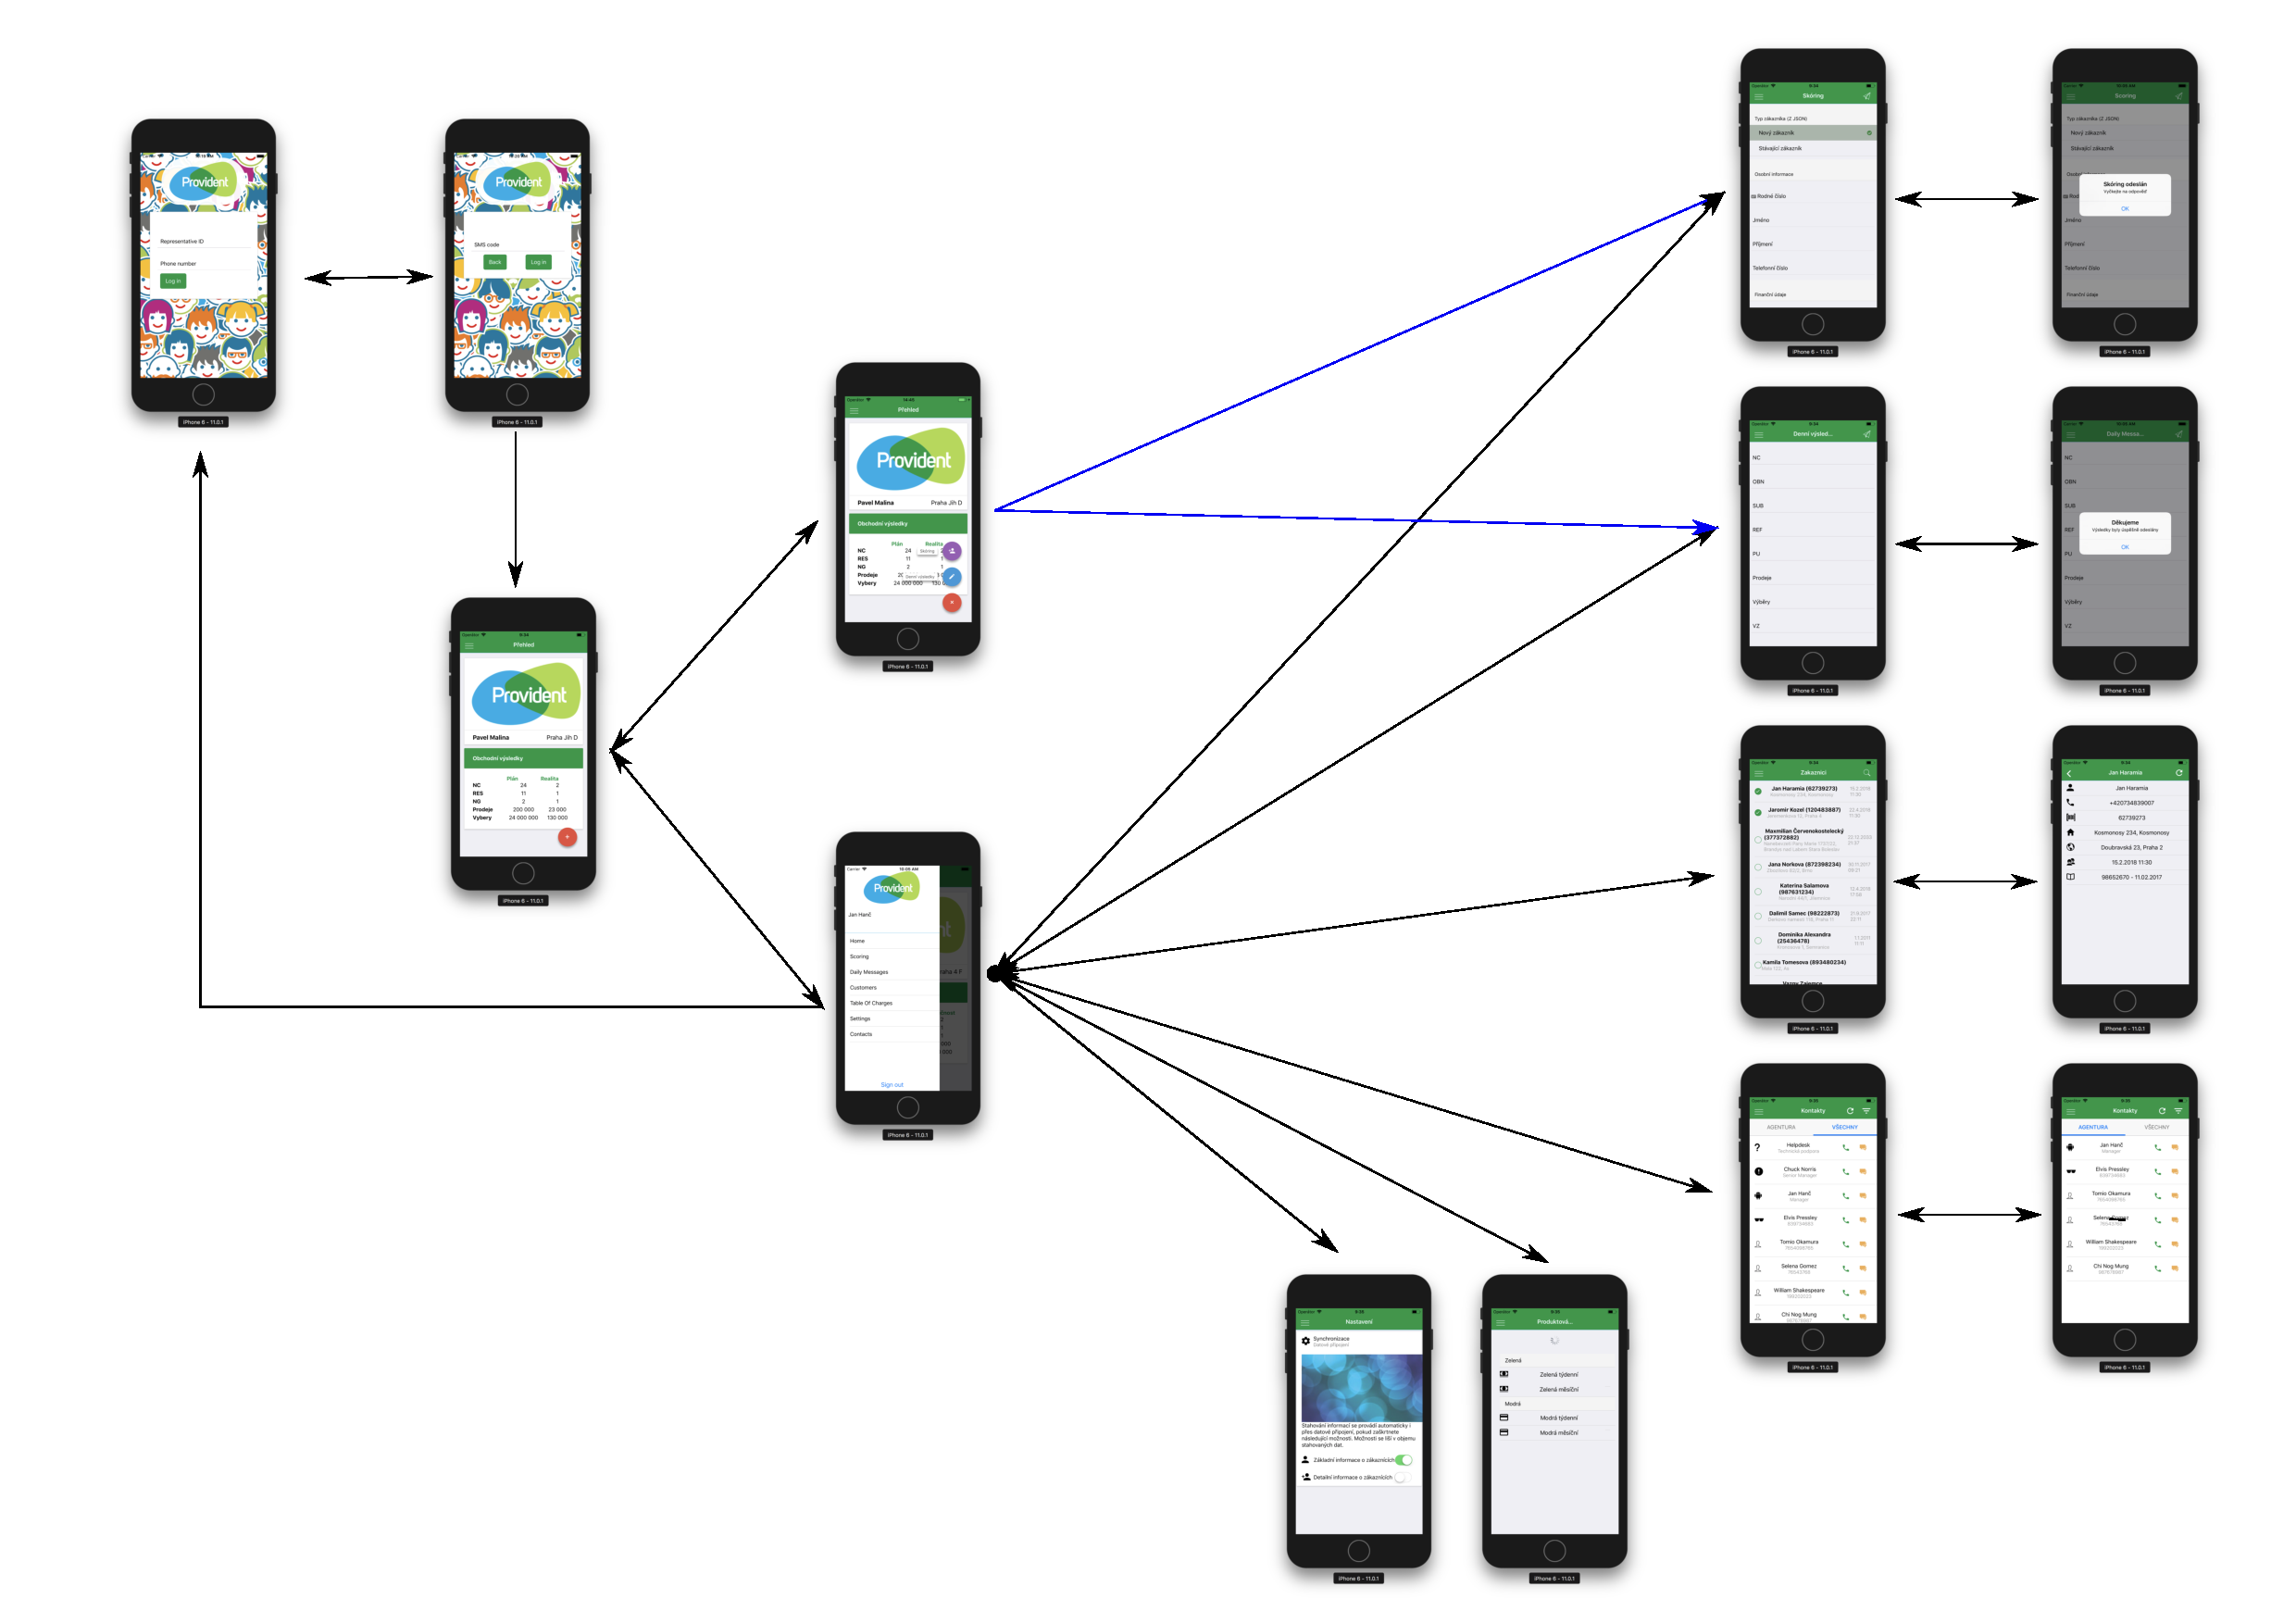
\includepdf[pages=1,clip,trim=2cm 1cm 21cm 1cm,noautoscale,fitpaper=false]{figures/screenflow.pdf}
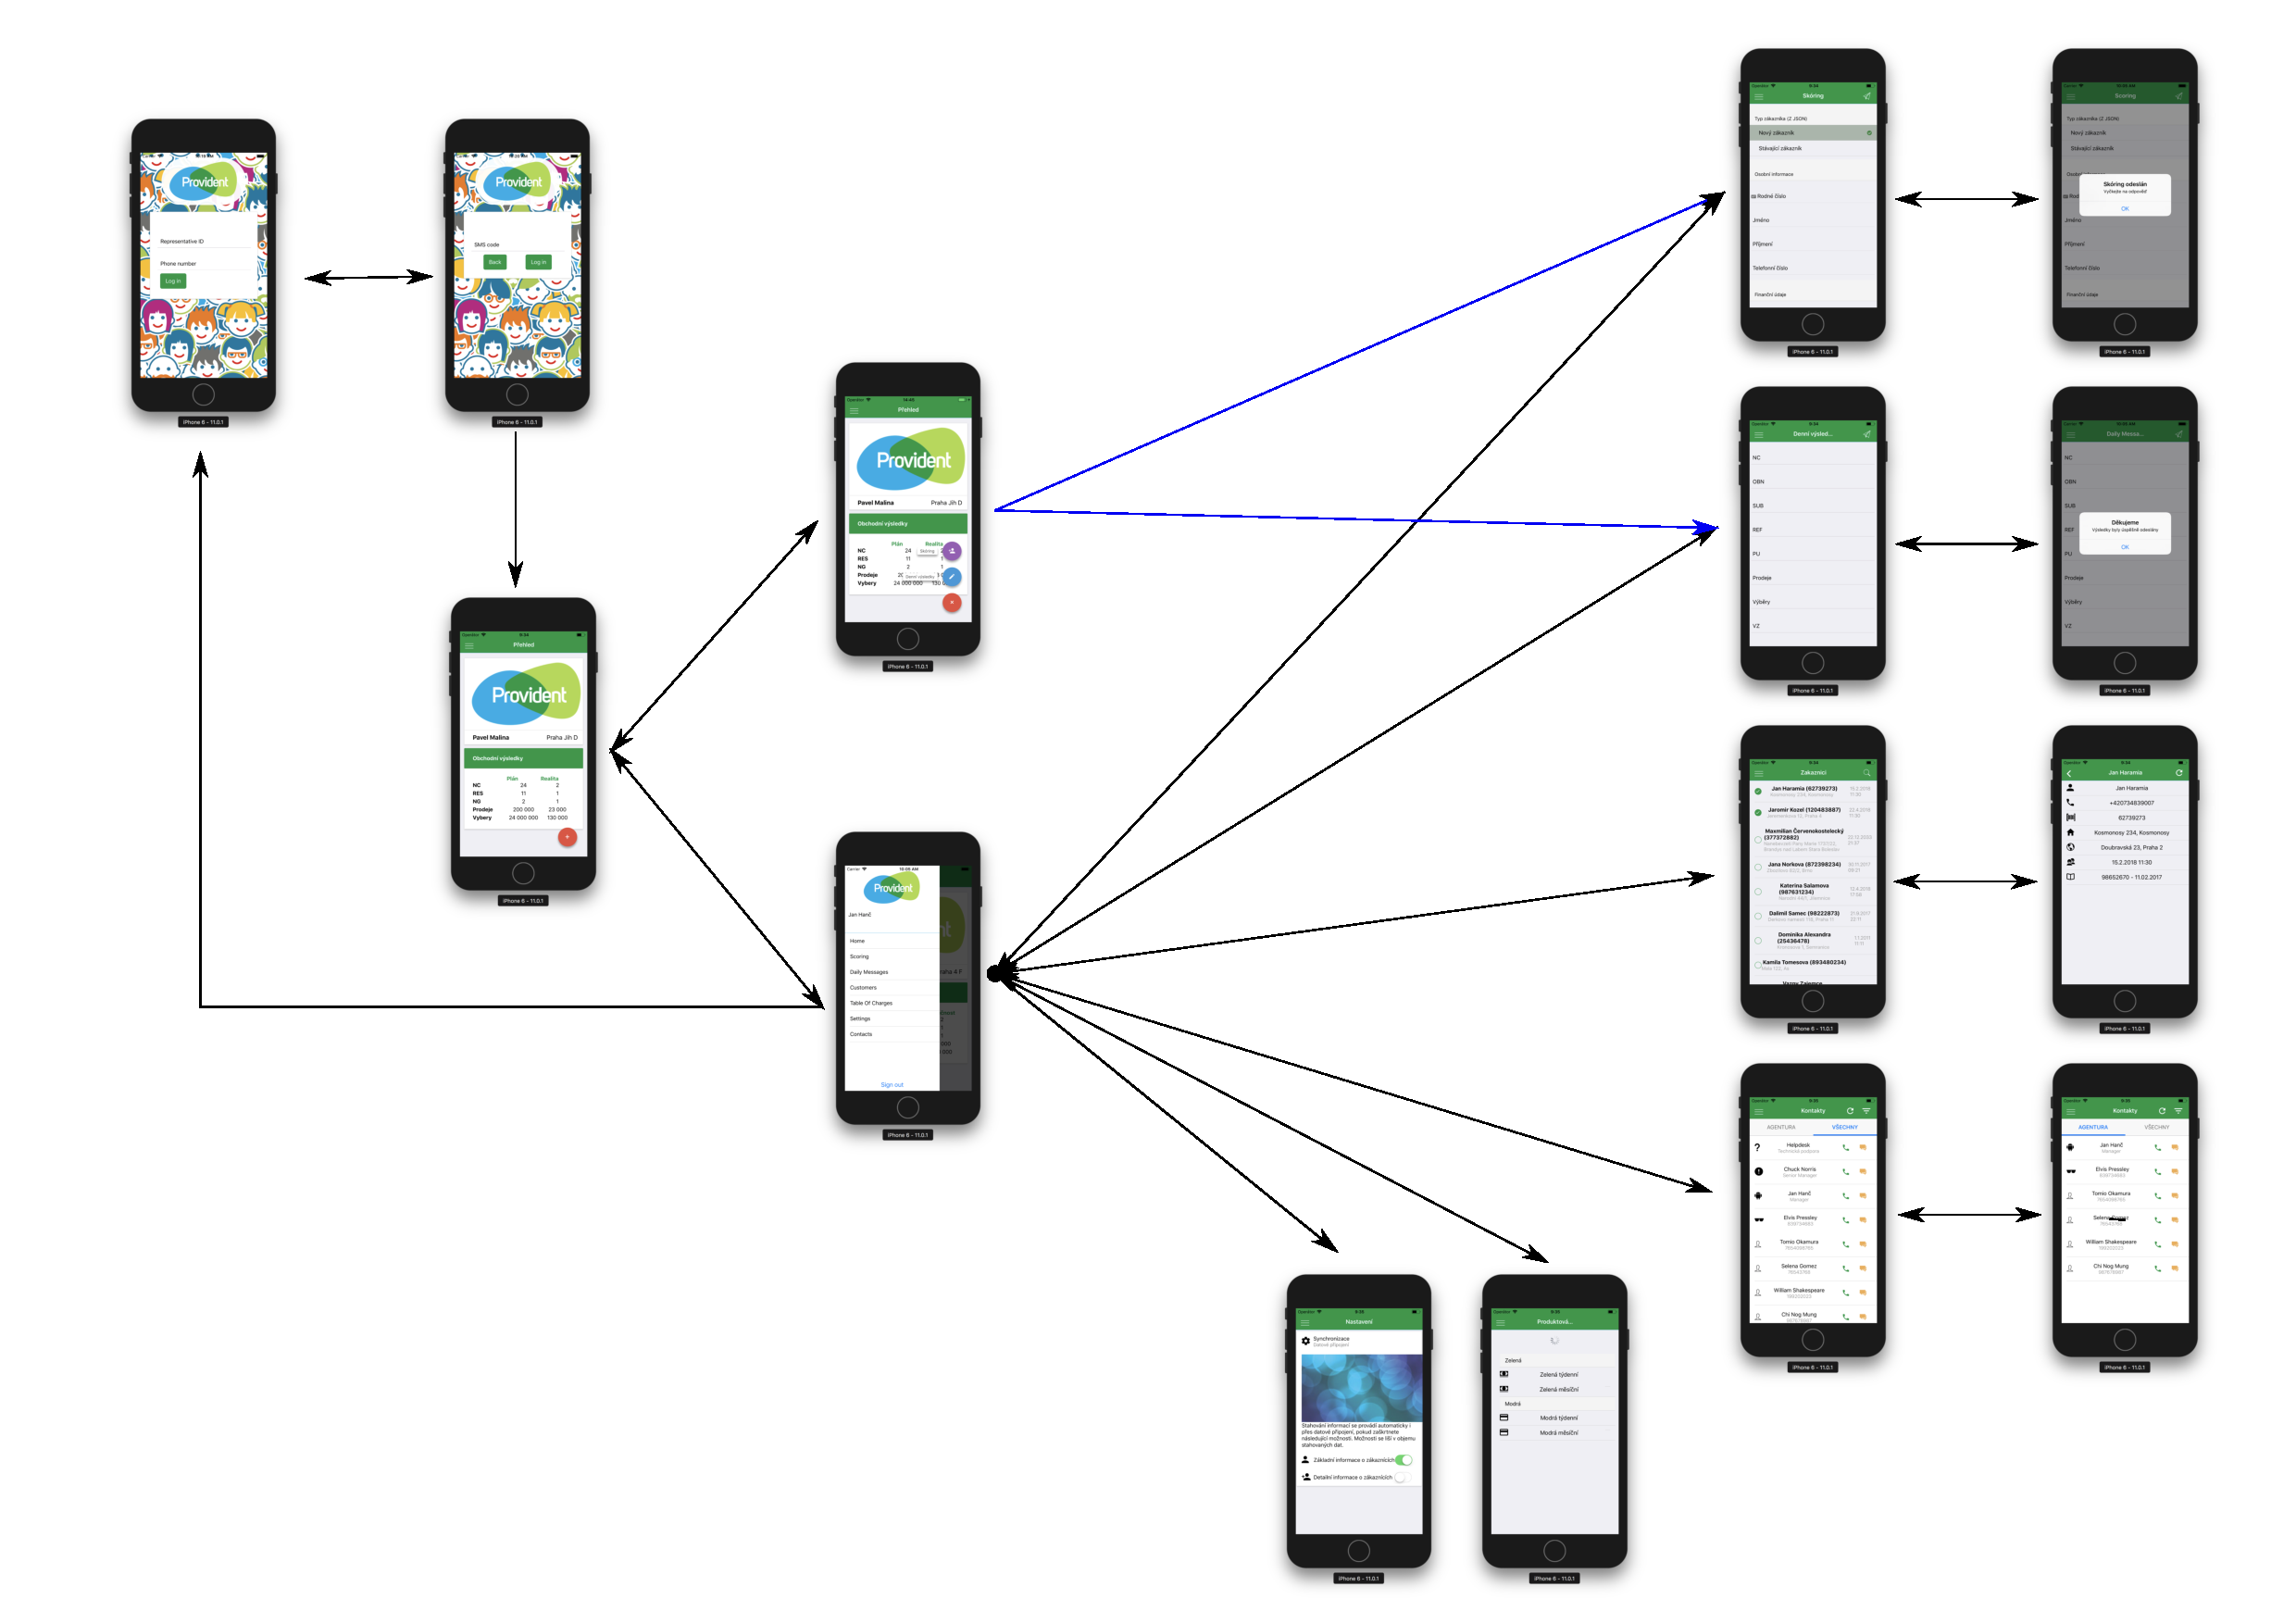
\includepdf[pages=1,trim=21cm 1cm 2cm 1cm,noautoscale,fitpaper=false]{figures/screenflow.pdf}

\end{document}
